%%
%% Copyright 2007, 2008, 2009 Elsevier Ltd
%%
%% This file is part of the 'Elsarticle Bundle'.
%% ---------------------------------------------
%%
%% It may be distributed under the conditions of the LaTeX Project Public
%% License, either version 1.2 of this license or (at your option) any
%% later version.  The latest version of this license is in
%%    http://www.latex-project.org/lppl.txt
%% and version 1.2 or later is part of all distributions of LaTeX
%% version 1999/12/01 or later.
%%
%% This template has been modified by Philip Blakely for
%% local distribution to students on the MPhil for Scientific
%% Computing course run at the University of Cambridge.
%%

%% Template article for Elsevier's document class `elsarticle'
%% with numbered style bibliographic references
%% SP 2008/03/01
%%
%%
%%
%% $Id: elsarticle-template-num.tex 4 2009-10-24 08:22:58Z rishi $

\documentclass[final,3p,times,twocolumn]{elsarticle}
\usepackage{pdfpages}
\usepackage{booktabs} % Tables
\usepackage{pifont}
\usepackage{placeins}
\usepackage{afterpage}

%% Use the option review to obtain double line spacing
%% \documentclass[preprint,review,12pt]{elsarticle}

%% Use the options 1p,twocolumn; 3p; 3p,twocolumn; 5p; or 5p,twocolumn
%% for a journal layout:
%% \documentclass[final,1p,times]{elsarticle}
%% \documentclass[final,1p,times,twocolumn]{elsarticle}
%% \documentclass[final,3p,times]{elsarticle}
%% \documentclass[final,3p,times,twocolumn]{elsarticle}
%% \documentclass[final,5p,times]{elsarticle}
%% \documentclass[final,5p,times,twocolumn]{elsarticle}

%% if you use PostScript figures in your article
%% use the graphics package for simple commands
%% \usepackage{graphics}
%% or use the graphicx package for more complicated commands
%% \usepackage{graphicx}
%% or use the epsfig package if you prefer to use the old commands
%% \usepackage{epsfig}

%% The amssymb package provides various useful mathematical symbols
\usepackage{amssymb}
\usepackage{float}
\usepackage{subfig}
\usepackage{graphicx}

%% Font setting, for my own eyes
\usepackage{libertine}
\usepackage{libertinust1math}
\usepackage[T1]{fontenc}

%% Algorithms
\usepackage[ruled,vlined]{algorithm2e}

%% Some math characters
\usepackage{bbold}

%% So that references are listed in the Contents
\usepackage[nottoc,notlot,notlof]{tocbibind}

\newcommand{\cmark}{\ding{51}}%
\newcommand{\xmark}{\ding{55}}%

%% The amsthm package provides extended theorem environments
%% \usepackage{amsthm}

%% The lineno packages adds line numbers. Start line numbering with
%% \begin{linenumbers}, end it with \end{linenumbers}. Or switch it on
%% for the whole article with \linenumbers after \end{frontmatter}.
%% \usepackage{lineno}

%% natbib.sty is loaded by default. However, natbib options can be
%% provided with \biboptions{...} command. Following options are
%% valid:

%%   round  -  round parentheses are used (default)
%%   square -  square brackets are used   [option]
%%   curly  -  curly braces are used      {option}
%%   angle  -  angle brackets are used    <option>
%%   semicolon  -  multiple citations separated by semi-colon
%%   colon  - same as semicolon, an earlier confusion
%%   comma  -  separated by comma
%%   numbers-  selects numerical citations
%%   super  -  numerical citations as superscripts
%%   sort   -  sorts multiple citations according to order in ref. list
%%   sort&compress   -  like sort, but also compresses numerical citations
%%   compress - compresses without sorting
%%
%% \biboptions{comma,round}

% \biboptions{}

\journal{MPhil in Scientific Computing}

\begin{document}
	
	\begin{frontmatter}
		
		%% Title, authors and addresses
		
		%% use the tnoteref command within \title for footnotes;
		%% use the tnotetext command for the associated footnote;
		%% use the fnref command within \author or \address for footnotes;
		%% use the fntext command for the associated footnote;
		%% use the corref command within \author for corresponding author footnotes;
		%% use the cortext command for the associated footnote;
		%% use the ead command for the email address,
		%% and the form \ead[url] for the home page:
		%%
		%% \title{Title\tnoteref{label1}}
		%% \tnotetext[label1]{}
		%% \author{Name\corref{cor1}\fnref{label2}}
		%% \ead{email address}
		%% \ead[url]{home page}
		%% \fntext[label2]{}
		%% \cortext[cor1]{}
		%% \address{Address\fnref{label3}}
		%% \fntext[label3]{}
		
		\title{Variational Monte Carlo (VMC) on a 3 dimensional model of \emph{Hookium}, a two electron harmonium in a Hooke’s potential, with parallelisation on a GPU}
		
		%% use optional labels to link authors explicitly to addresses:
		%% \author[label1,label2]{<author name>}
		%% \address[label1]{<address>}
		%% \address[label2]{<address>}
		
		\author{Bla\v z Stojanovi\v c}
		
		\address{Cavendish Laboratory, Department of Physics, J J Thomson
			Avenue, Cambridge. CB3 0HE}
		
		\begin{abstract}
			In this written assignment we implement a fully Variational Quantum Monte Carlo (VMC) code in order to study Hooke's-law atom (Hookium), a model in which the Coulomb interaction between the nucleus and electrons is replaced with a harmonic one. Numerically obtained ground state energies and position intracules are compared to analytical solutions in the special case of $k=\frac{1}{4}$. Alongside the VMC a variational Hartree-Fock method with Cartesian Gaussian basis functions is implemented, which permits calculations of the Correlation energy as well as aids in construction of trial wave functions used in the Monte Carlo method. The software is implemented in JAX, making it possible to run it on a GPU and evaluate gradients by using automatic differentiation. Energy and variance based optimisation is compared in the case of Hookium and correlation energies are calculated for a range of $k$'s. 
		\end{abstract}
	\end{frontmatter}
	
	%%
	%% Start line numbering here if you want
	%%
	%% \linenumbers
	
	\tableofcontents
	
	%% main text
	\section{Introduction}
	\label{sec:intro}
	The Schr{\"o}dinger equation underpins a large part of quantum chemistry and solid state physics. However, the quantum many-body problem, which amounts to solving the $3N$-dimensional Schr\"odinger equation is notoriously hard to solve. Ever since the postulation of the equation in 1925, great efforts have been made in solving the equation, both analytically and numerically. Perhaps most impactful was the development of various approximate methods to solve the many-body problem with the available computational resources. Hartree-Fock (HF) approaches solve an auxiliary system of independent electrons in a self-consistent field and assume that the wave function (for fermions) can be represented as a single Slater determinant. The HF method does not include electron correlation, which makes it a good approximation only in systems where correlation contributions are small. Post-Hartree-Fock methods, such as Coupled Cluster, Configuration interaction and M\o ller-Plesset theory include correlation by considering a linear combination of determinants, they can be extremely accurate but come at a high computational cost. 

	One of the most popular approaches used today is Density Functional Theory (DFT). It reformulates the many-body electron problem in terms of the $3$-dimensional electron density $n(\mathbf{r})$, which is found by minimising the total energy functional $E[n(\mathbf{r})]$~\cite{hohenberg1964inhomogeneous}. DFT provides an alternative line of thought to the truncated Hilbert space of single particle orbitals~\cite{kohn1999nobel} and is used extensively for simulating large systems as linear scaling variants of DFT exist~\cite{skylaris2005introducing}. 
	While DFT is theoretically exact the true energy functional $E[n(\mathbf{r})]$ is not known and its parameterisations employ more accurate \emph{ab initio} methods. One of which being Quantum Monte Carlo (QMC).
	
	\subsection{Quantum Monte Carlo methods}
	\label{subsec:intro-QMC}
	%% General about QMC
	Quantum Monte Carlo is a class of methods that use statistical sampling to directly deal with high-dimensional integration that arises from working with the many-body wave function. QMC methods are among the most accurate achieving chemical accuracy for smaller systems~\cite{foulkes2001quantum}, and can achieve any degree of statistical precision sought. Quantum Monte Carlo is also very versatile and can be applied at both zero and finite temperatures~\cite{austin2012quantum}.	
	%% Zero temperature methods
	%% Variational quantum monte carlo
	The most basic zero temperature QMC method is variational QMC (VMC). The method is composed of two parts, firstly it directly evaluates the variational energy $E_V = \langle \Psi_{T} | \hat H | \Psi_{T} \rangle / \langle \Psi_{T} | \Psi_{T} \rangle$ of the system using Monte Carlo integration and a trial wave function $\Psi_{T}$. Secondly the parameters of the trial wave function are optimised such as to minimise the variational energy $E_V$, giving the method its name. The first application of VMC was to ground state ${}^4$He~\cite{mcmillan1965ground}, it was later extended for studying many-body fermionic systems~\cite{ceperley1977monte}. A way of obtaining excitation energies using VMC is to use a trial wave function that models an excited state of the system, if the trial wave function obeys a certain symmetry, the variational principle guarantees that this VMC energy calculation gives an upper bound on the lowest exact eigenstate of this symmetry. Furthermore, the method can be extended to study non-equilibrium properties of bosonic~\cite{carleo2012localization, carleo2014light}, and fermionic~\cite{ido2015time} systems. The main advantage of VMC is its simplicity while the main drawback is that the accuracy is limited by the flexibility and form of the trial wave function~\cite{austin2012quantum}. As such VMC is usually employed as a first step in more advanced QMC simulations. 
		
		%% Green function QMC and Diffusion QMC
		Projector quantum Monte Carlo (PMC), is a class of QMC methods which are in essence nothing more than stochastic implementations of the power method to obtain the dominant eigenvector of a matrix or a kernel function~\cite{gubernatis_kawashima_werner_2016}. Their distinct advantage over VMC is that they are not constrained by our parametrisation of the trial wave function, as they can describe arbitrary probability distributions. The projector $\hat P$ has to be chosen in such a way, that the ground state of the system becomes the dominant eigenvector, i.e. $| \Psi_{0}\rangle = \lim_{n\rightarrow \infty} \hat{P}^n |\Psi_{T}\rangle$. Different ways of achieving this, the space (real or orbital space) in which the walk is done and choosing either first or second quantisation description, give rise to different flavours of PMC methods. Using an exponential projector $\hat{P} = e^{\tau (E_T \mathbb{1} - \hat{H})}$ can be interpreted as propagation in imaginary time $\tau \rightarrow it$ in turn transforming the Schr\"odinger equation into a diffusion equation, which is a continuous limit of the random walk and lends itself to stochastic integration~\cite{reynolds1990diffusion}. 
		Directly sampling from the exact Green function is known as Projector Green Function Monte Carlo (GFMC) method~\cite{kalos1962monte, kalos1966stochastic}. A convenient approximation to GFMC is its short-time approximation which leads to one of the most popular QMC methods, diffusion Monte Carlo (DMC)~\cite{foulkes2001quantum, reynolds1990diffusion}. In this regime one can exploit analytical solutions to diffusion and rate problems to write an explicit form of the Green's function. Additionally, by using the Trotter-Suzuki formula time-step bias can be expressed and accounted for~\cite{austin2012quantum}. DMC is statistically implemented by using a population of walkers which either branch or die, the average over all walkers is calculated. Reptation quantum Monte Carlo~\cite{reynolds1990diffusion} (RMC) is an alternative formulation which only uses a single walker, and instead of branching and dying the MC moves mutate the path of that single walker. The use of a guiding wave function for importance sampling greatly improves the statistical efficiency of PMC methods, the guiding wave function is usually obtained by means of VMC or some mean field calculation. 
		
		PMC method suffer from the \emph{sign problem}, which is present in Markov chain simulation of distributions that are not strictly positive, this is the case in fermionic and frustrated systems~\cite{gubernatis_kawashima_werner_2016}. The problem refers to an exponential decrease in sampling efficiency with system size. The search for solutions of this problem is still an area of active research~\cite{foulkes2001quantum} but is in practice remedied by the \emph{fixed-node} approximation~\cite{anderson1975random}. In it a boundary condition is imposed into the projection, such that the projected state shares the same zero crossings (nodal surface) with a trial wave function, which is again usually obtained with VMC. The projected state is now only exact when the nodal surface is exact, nevertheless this approximation is quite accurate~\cite{foulkes2001quantum}. Fixed node is widely used, one of its first applications was to the electron gas~\cite{ceperley1980ground}, which is used in parameterisations of the  exchange correlation functional in LSDA~\cite{vosko1980accurate}.
	
	%% Finite temperature methods
		Quantum Monte Carlo methods have had a lot of success at finite temperatures. Auxiliary-field Monte Carlo, or Path Integral Monte Carlo~\cite{ceperley1995path}, which leads to ring-polymer molecular dynamics, may be used for this purpose. Additionally QMC is not limited to continuum space applications and has been extensively used to study lattice models, notable examples being the cluster/loop algorithm and the worm algorithm~\cite{gubernatis_kawashima_werner_2016, prokof1998exact}.
	
	%% Computational considerations
		Quantum Monte Carlo methods are generally more computationally expensive than DFT approaches, but on the other hand QMC codes are, as a rule of thumb, simpler to implement. Furthermore, since the wave function does not need to be stored directly QMC has reasonable storage requirements. The high computational cost of the QMC methods is remedied by the fact that they are intrinsically parallelisable, the core calculation involves generating (pseudo)-random numbers, performing a simple calculation and in the end averaging over the results. Therefore, implementations of QMC algorithms that have been applied to practical problems are optimised to run on massively parallel hardware with little overhead~\cite{needs2020variational}. Finally, the repetitive nature of the Monte Carlo calculation lends itself to hardware acceleration using either graphical processing units (GPUs) or field-programmable gate arrays (FPGAs)~\cite{austin2012quantum}.
		
		
	\subsection{Graphical processing units}
	%% In general about GPUs in science, especially as it comes to applications in quantum chemistry ~300 besed
	Building customised hardware for graphics is common practice since the 1970s, but the term \emph{graphical processing unit} (GPU) as we know it today was popularised at the turn of the millennium by NVIDIA. GPUs were originally designed with very specialised tasks in mind, but in the last two decades there has been an in increased interest in leveraging GPU for various computationally intensive applications, usually referred to as \emph{general-purpose computing on graphical processing units} (GPGPU). The main advantage of graphical processing units over CPUs is higher theoretical \emph{floating point operations per second} (FLOPS) and increased theoretical bandwidth. This is achieved by dedicating a larger proportion of transistors in the processing unit to data processing as opposed to flow control and data catching, as well as not performing branch checking~\cite{cuda}, see Figure~\ref{fig:cuda-gpu}.
	% TODO: \usepackage{graphicx} required
	\begin{figure}[h]
		\centering
		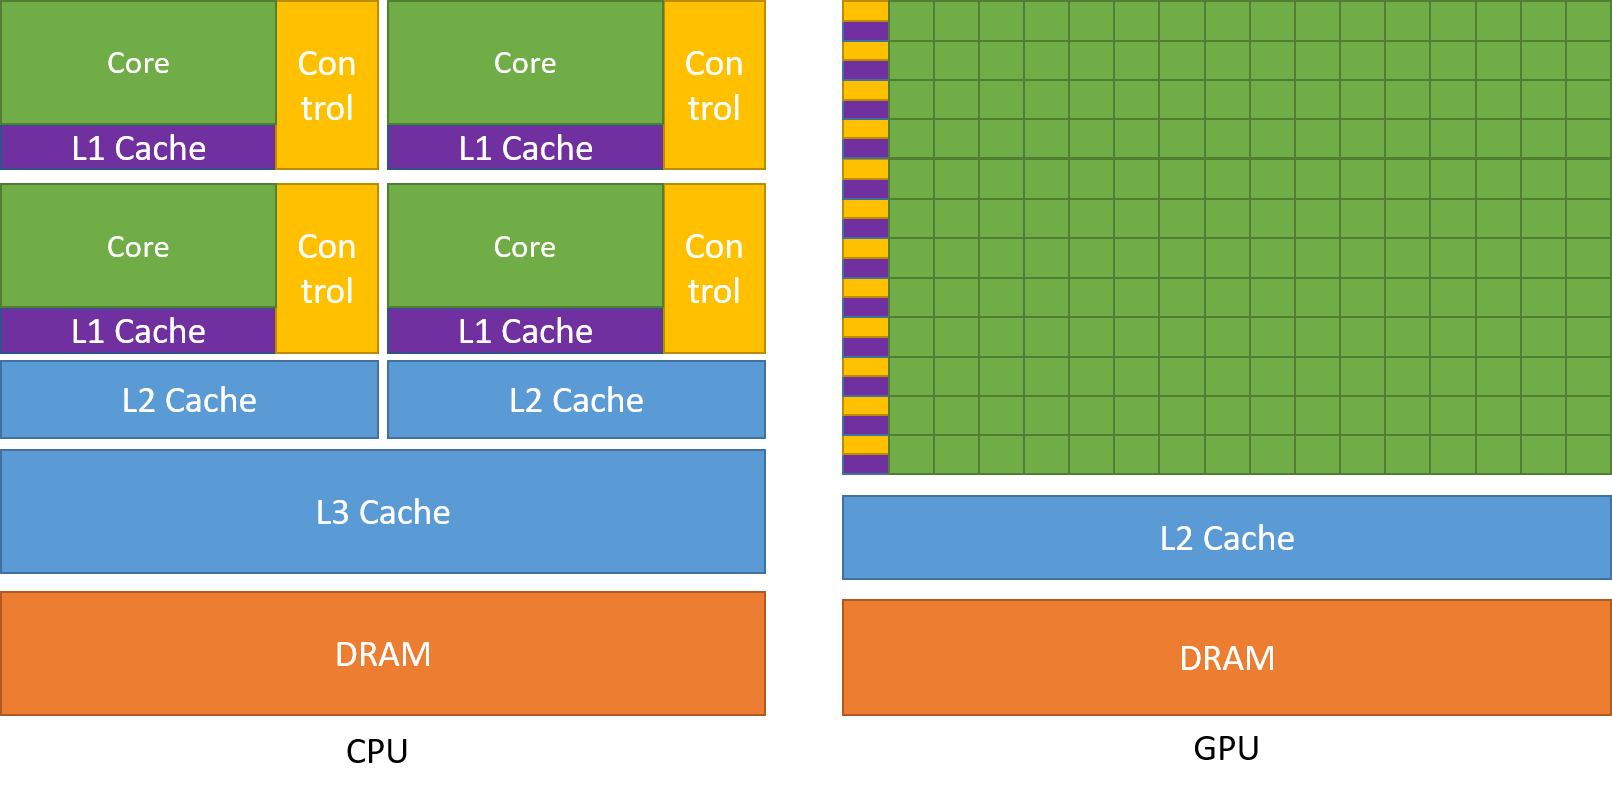
\includegraphics[width=\linewidth]{../diagrams/cuda-gpu}
		\caption{A comparison of a CPU and GPU, from~\cite{cuda}.}
		\label{fig:cuda-gpu}
	\end{figure}
	% how do they work?
	GPUs were designed to work with small fragments of data (pixels) and perform the same operation many times simultaneously on all of the fragments. In the CUDA parallel programming model the problem at hand is required to be decomposable into tasks that can be independently executed in parallel by \emph{blocks} of \emph{threads}. The tasks must be such that they can be executed in parallel by the threads within a block. Each thread executes functions called \emph{kernels}. A substantial speedup of a calculation can be achieved \emph{if} it can be made to comply with the data and thread parallelism required for the above described procedure. 
	
	QMC methods can be made to fit this mold and there has been extensive work done in this direction~\cite{anderson2007quantum, meredith2009accuracy, esler2010accelerating}. GPUs can be exploited by initializing multiple walkers and running them in parallel thread blocks before averaging the results over all of them. Additionally GPUs can be used to accelerate the evaluation of basis function expansions, the linear algebra associated with computing the Slater determinant and evaluation of complicated forms of the Jastrow factor in Variational Monte Carlo. Since most GPUs only support single precision arithmetic, accuracy was of concern in first applications to QMC, benchmarks have shown that chemical accuracy is still achievable on GPUs~\cite{anderson2007quantum, meredith2009accuracy}. 
	
	
	\subsection{Hookium}
	%% Very quick introduction to Hookium
	We can construct a toy model of two electrons that resembles the helium atom, where the electrons are bound to the nucleus with a harmonic instead of a Coulomb potential. 
	\begin{figure}[h]
		\centering
		\includegraphics[width=0.35\linewidth]{../diagrams/Hookium/Hookium_diagram}
		\caption{Hookium atom, two electrons that are bound to the nucleus with springs of coefficient $k$ and interact via the Coulomb force.}
		\label{fig:Hookiumdiagram}
	\end{figure}
	The Hamiltonian of the model is then defined as 
	\begin{equation}
		\hat{H}=-\frac{1}{2} \nabla_{1}^{2}-\frac{1}{2} \nabla_{2}^{2}+\frac{1}{2} k r_{1}^{2}+\frac{1}{2} k r_{2}^{2}+\frac{1}{r_{12}}.
	\end{equation}
	This model is referred to as \emph{Hookium} (sometimes Harmonium). Although it is quantitatively different from helium some meaningful qualitative comparisons can be made~\cite{ONeill2003wave}. Most notably Hookium has an analytical solution for the case $k=\frac{1}{4}$, making it an ideal candidate to benchmark computational methods, which is the topic of this written assignment. The normalized closed form wave function solution of the ground state in position space is
	\begin{equation}
		\Psi\left(\mathbf{r}_{1}, \mathbf{r}_{2}\right)=\frac{1}{2 \sqrt{8 \pi^{5 / 2}+5 \pi^{3}}}\left(1+\frac{r_{12}}{2}\right) \exp \left(-\frac{r_{1}^{2}+r_{2}^{2}}{4}\right), 
	\end{equation}
	the energy of the state is $E=2$. 
	The probability of finding two electrons distance $u$ apart; the position intractule $P(u)$, is also useful. It is defined as
	\begin{equation}
		P(u)=\iiint\left|\Psi\left(\mathbf{r}_{1}, \mathbf{r}_{2}\right)\right|^{2} \delta\left(\mathbf{r}_{12}-\mathbf{u}\right) d \mathbf{r}_{1} d \mathbf{r}_{2} d \Omega_{\mathbf{u}},
	\end{equation}
	for Hookium it too has a closed form
	\begin{equation}
		P(u)=\frac{1}{8+5 \pi^{1 / 2}} u^{2}\left(1+\frac{u}{2}\right)^{2} \exp \left(-\frac{u^{2}}{4}\right).
	\end{equation}
	Values of $h=m=c=1$ and $1E_h = 1$ will be assumed throughout this report. 
	Hookium will be studied with the VMC method and the above expressions will be used to compare the accuracy of the numerical method.
	
	The rest of this written assignment is structured as follows. In section~\ref{sec:impl}, the details necessary to implement the variational Monte Carlo method are presented. Additionally details of GPU acceleration and parallelisation of the method are discussed. Presentation of numerical results and benchmarks of the method follow in section~\ref{sec:results}. The final section~\ref{sec:conclusion} contains a short conclusion and proposals for further work. 
	\section{Implementation}
	\label{sec:impl}
	
	\subsection{Monte Carlo Importance Sampling}
	\label{subsec:Impl-MCIP}
	The most common application of Monte Carlo methods is evaluation of integrals in high dimensional space. There MC has a distinct advantage over quadrature methods, as the statistical error decreases with the square root of samples irregardless of the dimensionality of the problem. Integrals of a function $g(\mathbf{R})$
	\begin{equation}
		I=\int g(\mathbf{R}) \mathrm{d} \mathbf{R},
	\end{equation}
	where $\mathbf{R}$ is the \emph{configuration} of the system or simply a \emph{walker}, can be integrated by use of an \emph{importance function} $\mathrm{P}(\mathbf{R})$, where $\int d \mathbf{R} \text{P}(\mathbf{R})=1$ and $\mathrm{P} (\mathbf{R}) \geq 0$. The integral can be rewritten in the form
	\begin{equation}
		\int g(\mathbf{R}) \mathrm{d} \mathbf{R} = \int \frac{g(\mathbf{R})}{\mathrm{P}(\mathbf{R})} \mathrm{P}(\mathbf{R}) \mathrm{d} \mathbf{R} = \int f(\mathbf{R})\mathrm{P}(\mathbf{R}) \mathrm{d} \mathbf{R},
	\end{equation}
	where $f(\mathbf{R}) = g(\mathbf{R}) / \mathrm{P}(\mathbf{R})$.
	The importance function $\mathrm{P}(\mathbf{R})$ can be interpreted as a probability density. If we now generate an infinite number of random uncorrelated configurations $\mathbf{R}_m$ from the distribution $\mathrm{P}(\mathbf{R})$, the sample average is a good estimator of the integral $I$
	\begin{equation}
		I=\lim _{M \rightarrow \infty}\left\{\frac{1}{M} \sum_{m=1}^{M} f\left(\mathbf{R}_{m}\right)\right\},
	\end{equation}
	and for an approximation with a finite number of samples
	\begin{equation}
		I \approx \frac{1}{M} \sum_{m=1}^{M} f\left(\mathbf{R}_{m}\right).
	\end{equation}
	Under conditions where the central limit theorem holds~\cite{foulkes2001quantum}, the estimator is normally distributed with variance $\sigma_{f}^{2}/M$, which can also be estimated from the samples as
	\begin{equation}
		\frac{\sigma_{f}^{2}}{M} \approx \frac{1}{M(M-1)} \sum_{m=1}^{M}\left[f\left(\mathbf{R}_{m}\right)-\frac{1}{M} \sum_{n=1}^{M} f\left(\mathbf{R}_{n}\right)\right]^{2}.
	\end{equation}
	In the case of Hookium the configurations $\mathbf{R}$ are the positions of the electrons.
	
	\subsection{Metropolis-Hastings algorithm}
		\label{subsec:Impl-MCMC}
	The integration technique from the previous section relies on our ability to obtain samples from a probability distribution $\mathrm{P}(\mathbf{R})$. In the case of QMC these distributions are high-dimensional and cannot be directly sampled from, moreover their normalisations are usually not known. 
	The Metropolis-Hastings algorithm~\cite{hastings1970monte}, see Algorithm~1, avoids direct sampling from the distribution $\mathrm{P}(\mathbf{R})$ and is insensitive to its normalisation. It uses a Markov process whose stationary distribution $\pi(\mathbf{R})$ is the same as $\mathrm{P}(\mathbf{R})$	
	to generate a sequence of configurations $\left\{\mathbf{R}_n\right\}_\mathrm{P}$ 
	that are drawn from $\mathrm{P}(\mathbf{R})$. A Markov process is completely defined with its transition probability $\mathrm{P}(\mathbf{R} \rightarrow \mathbf{R}^\prime)$, which is the probability of transitioning from state $\mathbf{R}$ to state $\mathbf{R}^\prime$. For the process to have a unique stationary distribution two conditions must be met, the process must be \emph{ergodic} and it must obey \emph{detailed balance}
	\begin{equation}
		\mathrm{P}(\mathbf{R}) \mathrm P(\mathbf{R} \rightarrow \mathbf{R}^\prime) = \mathrm{P}(\mathbf{R}^\prime) \mathrm P(\mathbf{R}^\prime \rightarrow \mathbf{R}),
	\end{equation}
	rewritten as
	\begin{equation}
		\label{eq:detailed_balance}
		\frac{\mathrm P ({\mathbf{R}})}{\mathrm P ({\mathbf{R}^\prime})} = \frac{\mathrm P(\mathbf{R}^\prime \rightarrow \mathbf{R})}{\mathrm P(\mathbf{R} \rightarrow \mathbf{R}^\prime)}.
	\end{equation}
	The right transition probability $\mathrm P(\mathbf{R} \rightarrow \mathbf{R}^\prime)$ is not known, but we can express it with a trial move transition probability $\mathrm{T}(\mathbf{R} \rightarrow \mathbf{R}^\prime)$ which we sample and acceptance probability $\mathrm{A}(\mathbf{R} \rightarrow \mathbf{R}^\prime)$ as
	\begin{equation}
		\mathrm P(\mathbf{R} \rightarrow \mathbf{R}^\prime) = \mathrm T(\mathbf{R} \rightarrow \mathbf{R}^\prime) \mathrm A(\mathbf{R} \rightarrow \mathbf{R}^\prime).
	\end{equation}
	For equation~\eqref{eq:detailed_balance} to hold, the acceptance probability must be 
	\begin{equation}
		A\left(\mathbf{R} \rightarrow \mathbf{R}^{\prime}\right)=\min \left(1, \frac{\mathrm{T}\left(\mathbf{R}^{\prime} \rightarrow \mathbf{R}\right) \mathrm{P}\left(\mathbf{R}^{\prime}\right)}{\mathrm{T}\left(\mathbf{R} \rightarrow \mathbf{R}^{\prime}\right) \mathrm{P}(\mathbf{R})}\right).
	\end{equation}
	Thus to sample from any probability distribution we need only have the ability to calculate probabilities $\mathrm P(\mathbf{R})$ and to sample from a trial transition probability $\mathrm T(\mathbf{R} \rightarrow \mathbf{R}^{\prime})$. The efficiency of the algorithm depends on the amount of trial moves that we reject. All trial moves would be accepted if $\mathrm{T}(\mathbf{R} \rightarrow \mathbf{R}^{\prime})= \mathrm{P}(\mathbf{R}^\prime)$, which would just mean sampling from $\mathrm P$ directly and is the very problem we are trying to solve with Metropolis-Hastings. 	
	\begin{algorithm}
		\label{alg:MCMC}
		\SetAlgoLined
		\KwResult{A set of configurations $\left\{ \mathbf{R}_n \right\}_{\mathrm{P}}$ sampled from $\mathrm P$}
		Initialize walker at random configuration $\mathbf{R}$\;
		\While{no. samples less than $N$}{
			Generate new configuration $\mathbf{R}^\prime$ with transition probability $\mathrm{T}(\mathbf{R}\rightarrow\mathbf{R}^\prime)$\;
			
			Accept the move ($\mathbf{R} \rightarrow \mathbf{R}^\prime$) with probability $A\left(\mathbf{R} \rightarrow \mathbf{R}^{\prime}\right)=\min \left(1, \frac{\mathrm{T}\left(\mathbf{R}^{\prime} \rightarrow \mathbf{R}\right) \mathrm{P}\left(\mathbf{R}^{\prime}\right)}{\mathrm{T}\left(\mathbf{R} \rightarrow \mathbf{R}^{\prime}\right) \mathrm{P}(\mathbf{R})}\right)$\;
			
			Append $\mathbf{R}$ to the set of configuration;
			
		}
		\caption{Metropolis-Hastings}
	\end{algorithm}
	
	\subsection{Variational Quantum Monte Carlo}
	Variational quantum Monte Carlo uses a trial wave function $\Psi_{T}$ which is an approximation to the true ground state wave function to directly evaluate the expectation value of $\hat H$ which provides an upper bound on the ground state energy
	\begin{equation}
		\label{eq:variational_princ}
		E_{V}=\frac{\langle \Psi_{T} | H | \Psi_{T} \rangle}{\langle \Psi_{T} | \Psi_{T} \rangle}
		=\frac{\int \Psi_{T}^{*}(\mathbf{R}) \hat{H} \Psi_{T}(\mathbf{R}) d \mathbf{R}}{\int \Psi_{T}^{*}(\mathbf{R}) \Psi_{T}(\mathbf{R}) d \mathbf{R}} \geq E_{0}.
	\end{equation}
	The expression for the variational energy $E_V$ can be rewritten as
	\begin{equation}
		\label{eq:E_V}
		E_{V}=\frac{\int\left|\Psi_{T}(\mathbf{R})\right|^{2}\left(\Psi_{T}(\mathbf{R})^{-1} \hat{H} \Psi_{T}(\mathbf{R})\right) d \mathbf{R}}{\int\left|\Psi_{T}(\mathbf{R})\right|^{2} d \mathbf{R}}.
	\end{equation}
	The above integral is estimated by using Metropolis-Hastings to sample a set of configurations $\left\{ \mathbf{R}_n \right\}_{\mathrm{P}}$ from the probability distribution given by the (normalized) trial wave function as $\mathrm{P}(\mathbf{R}) = |\Psi_T(\mathbf{R})|^2 \mathrm{d}\mathbf{R}$ and averaging these \emph{local} $E_L$ contributions
	\begin{equation}
		E_{V} \approx \frac{1}{M} \sum_{m=1}^{M} E_{L}\left(\mathbf{R}_{m}\right),
	\end{equation}
	where
	\begin{equation}
		E_{L}(\mathbf{R})=\Psi_{T}(\mathbf{R})^{-1} \hat{H} \Psi_{T}(\mathbf{R}).
	\end{equation}
	The procedure is analogous for any other calculation of expectation value. Trial moves may be chosen in a variety of ways depending on the system studied, in the case of Hookium we will use a Gaussian distribution centered at the current position of the walker.
	
	Estimation of the variational energy $E_V$ is only one part of a variational Monte Carlo simulation. The second part is the variational optimisation of the trial wave function. The trial wave function $\Psi_T$ is parameterized with a set of variational parameters $\left\{\alpha_k\right\}$, historically the number of parameters has been low due to high computational cost~\cite{foulkes2001quantum}. The optimal parameters for the system are found by minimizing the \emph{cost function}. A straightforward choice of cost function is the variational energy $E_V$ in eq.~\eqref{eq:E_V}. Given that its value is bounded below due to the variational principle, eq~\eqref{eq:variational_princ}, its minimisation gives parameters $\left\{\alpha_k\right\}$ that give the best energy estimate for given parameterisation. An alternative is to minimize the variance of energy
	\begin{equation}
		\sigma_{E}^{2}(\left\{\alpha_k\right\})=\frac{\int \Psi_{T}^{2}(\left\{\alpha_k\right\})\left[E_{L}(\left\{\alpha_k\right\})-E_{V}(\left\{\alpha_k\right\})\right]^{2} d \mathbf{R}}{\int \Psi_{T}^{2}(\left\{\alpha_k\right\}) d \mathbf{R}},
	\end{equation}	
	this minimizes the statistical error of VMC estimation of energy. Most practical calculations are done by minimizing energy variance~\cite{foulkes2001quantum}. Minimisation of energy variance works because of the \emph{zero-variance} property, which is exclusive for quantum expectation values. If the trial wave function $\Psi_{T}$ is an exact eigenfunction of the Hamiltonian
	\begin{equation}
		\hat H |\Psi_{T}\rangle = E_V |\Psi_{T}\rangle,
	\end{equation}
	then the local energy $E_L$, a random variable, does not depend on the sampled configuration $\mathbf{R}$ 
	\begin{equation}				
		E_{L}(\mathbf{R})=\Psi_{T}(\mathbf{R})^{-1} \hat{H} \Psi_{T}(\mathbf{R}) = \Psi_{T}(\mathbf{R})^{-1} E_V \Psi_{T}(\mathbf{R}) = E_V,
	\end{equation}
	is constant and hence has zero variance. This equality holds only when $\Psi_{T}$ is an exact eigenfunction of the Hamiltonian. However, zero-variance property has important consequences for numerical stability of optimisation, it means that energy variance minima are robust to finite sampling. Minimizing the variance of energy drives the trial wave function towards eigenstates of the Hamiltonian. Moreover, the statistical error associated with estimation of any expectation value $\langle \hat O \rangle$ is proportional to the variance of $\hat O$, one can use the zero-variance condition to define a renormalized observable $\tilde O$ with the same average and smaller variance~\cite{assaraf1999zero} for more efficient sampling. 

	Various approaches to minimize the cost function can be taken, the simplest is trial and error using simple fitting procedures, this only works for small numbers of parameters. Alternatively a reweighting technique can be used to evaluate the energy or energy variance of a wave function with slightly different parameters $\Psi_{T}(\left\{\alpha + \delta \alpha\right\})$ to the one already evaluated $\Psi_{T}(\left\{\alpha\right\})$~\cite{umrigar1988optimized}, this increases the number of variational parameters that can be treated in small systems. Another option is to evaluate energy derivatives and use some sort of stochastic optimisation technique, \emph{stochastic gradient descent} being the simplest and \emph{stochastic recofiguration}~\cite{sorella1998green} being a more elaborate alternative. 
		
	\subsubsection{Trial wave functions $\Psi_{T}$}
	The choice of trial wave function $\Psi_{T}$ is the limiting factor for the performance of VMC, it determines its statistical efficiency and its final accuracy. The choice of trial wave function flexible but must satisfy the following conditions~\cite{foulkes2001quantum}; both the wave function and its gradient must be finite where the potential is finite, the wave function must have the appropriate symmetry and integrals 
	\begin{equation}
		\int \Psi_{T}^{*} \Psi_{T}, \quad \int \Psi_{T}^{*} \hat{H} \Psi_{T} \quad \text{and} \quad \int \Psi_{T}^{*} \hat{H}^{2} \Psi_{T}
	\end{equation}
	must exist. A popular choice and the one we will use in this project is the \emph{Slater-Jastrow} state. The trial wave function is a product of a Slater determinant $D(\mathbf{R})$ of single particle states $\left\{\psi_k(\mathbf{r})\right\}$ 
	\begin{equation}
		D(\mathbf{X}) = \frac{1}{\sqrt{N !}}\left|\begin{array}{cccc}\psi_{1}\left(\mathbf{x}_{1}\right) & \psi_{2}\left(\mathbf{x}_{1}\right) & \cdots & \psi_{N}\left(\mathbf{x}_{1}\right) \\ \psi_{1}\left(\mathbf{x}_{2}\right) & \psi_{2}\left(\mathbf{x}_{2}\right) & \cdots & \psi_{N}\left(\mathbf{x}_{2}\right) \\ \vdots & \vdots & \ddots & \vdots \\ \psi_{1}\left(\mathbf{x}_{N}\right) & \psi_{2}\left(\mathbf{x}_{N}\right) & \cdots & \psi_{N}\left(\mathbf{x}_{N}\right)\end{array}\right|
	\end{equation}	
	and the \emph{Jastrow correlation factor} $J(\mathbf{X})$
	\begin{equation}
		\Psi_{SJ}(\mathbf{X})=e^{J(\mathbf{X})} D(\mathbf{X}),
	\end{equation}
	where $\mathbf{X}$ is a configuration that contains both the spin and position degrees of freedom $\mathbf{x}_i = (\mathbf{r}_i, s_i)$. The discriminant is usually decomposed into spin up and down components as
	\begin{equation}
		D(\mathbf{X}) = D^{\uparrow}\left(\mathbf{r}_{1}, \ldots, \mathbf{r}_{N_{\uparrow}}\right) D^{\downarrow}\left(\mathbf{r}_{N_{\uparrow}+1}, \ldots, \mathbf{r}_{N}\right),
	\end{equation}
	this is computationally beneficial as it results in smaller determinants and no explicit sum over spin.
	The Jastrow factor is heuristically constructed to incorporate electron correlation into the wave function. In most practical calculations it is limited to one- and two-body terms~\cite{foulkes2001quantum}
	\begin{equation}
		\label{eq:jast}
		J(\mathbf{R})=
		\underbrace{\sum_{i=1}^{N} \chi\left(\mathbf{r}_{i}\right)}_{\text{one-body}}
		-
		\underbrace{\frac{1}{2} \sum_{i=1}^{N} \sum_{j<i}^{N} u\left(\mathbf{r}_{i}, \mathbf{r}_{j}\right)}_{\text{two-body}}.
	\end{equation}
	The first term describes the nuclear-electronic correlation and the second electron-electron correlation, in this project we will focus only on the second term. 
	Various forms of $u(\mathbf{r}_{i}, \mathbf{r}_{j})$ exist depending on application area, a common form for atomic and molecular calculations is
	\begin{equation}
		\label{eq:u}
		u(r_{ij})=\frac{a_{ij} r_{ij}}{1+\sum_{\kappa=1} b^{(\kappa)}_{ij} r^\kappa_{ij}}
	\end{equation}
	The parameters $a_{ij}$ are chosen to satisfy the \emph{cusp conditions},  
	\begin{equation}
		\left.\frac{d u}{d r}\right|_{r=0}=\left\{\begin{array}{cl}-\frac{1}{2}, & \text { for opposite spins, } \\ -\frac{1}{4}, & \text { for parallel spins. }\end{array}\right.
	\end{equation}
	and the $b^{(\kappa)}_{ij}$ parameters remain to be optimised variationally. 
	
	\subsubsection{Basis sets}
	There are various choices of single particle states $\left\{\psi_k(\mathbf{r})\right\}$ that compose the Slater determinant. They can be obtained from less expensive electronic structure methods, popular choices being LDA or HF, they can be from a standard basis set, such as atomic orbitals, Gaussian or plane wave sets, or they can be designed for the particular case at hand. In this work, we will compare performance of HF orbitals obtained from Cartesian Gaussian-type orbitals (GTOs)
	\begin{equation}
	\label{eq:cartG}
	G_{i j k}(\mathbf{r}, \alpha, \mathbf{A})=(x-x_{A})^{i} (y-y_{A})^{j} (z-z_{A})^{k} e^{-\alpha r_{A}^{2}},
	\end{equation}
	and HF orbitals obtained from the harmonic oscillator basis set
	\begin{equation}
		\phi_{k}(r)=\frac{H_{2 k-1}(r / \sqrt{2})}{2^{k} \sqrt{(2 k-1) !} r / \sqrt{2}} \frac{\exp \left(-r^{2} / 4\right)}{(2 \pi)^{3 / 4}}.
	\end{equation}
	Both basis sets and implementation of Hartree-Fock are discussed in more detail in~\ref{app:basissets} and~\ref{app:HF}.  
	
	\begin{figure*}[h]
		\vspace*{-2cm}
		\makebox[\linewidth]{
			
\includegraphics[width=1.3\textwidth]{../diagrams/Software/software_diagram.pdf}
		}
		\caption{Diagram of the general software framework developed to solve the Hookium atom with VMC. It is comprised of two modules, that need not be used together. Both the $a)$ Hartree-Fock and $b)$ the VMC module are variational and allow for rich variational approaches to a particular problem.}
		\label{fig:software}
	\end{figure*}
	
	\subsubsection{Generating trial moves}
	When proposing trial moves, we would like to minimize the correlation between subsequent states $\mathbf{R}$ and $\mathbf{R}^\prime$ as well as maximize the acceptance probability $A(\mathbf{R} \rightarrow \mathbf{R}^{\prime})$. Trial move probability determines both the size and average acceptance of the moves, practice we seek a compromise between both. First proposal probabilities were symmetric, meaning that the acceptance probability factors into
	\begin{equation}
		A\left(\mathbf{R} \rightarrow \mathbf{R}^{\prime}\right)=\min \left(1, \frac{\mathrm{P}(\mathrm{R}^{\prime})}{\mathrm{P}(\mathrm{R})}\right) = \min\left(1, \frac{|\Psi(\mathbf{R}^\prime)|^2}{|\Psi(\mathbf{R})|^2}\right).
	\end{equation}
	However it is beneficial to use information from the probability distribution to aid sampling. A common choice of non-symmetric trial move probability and the one we will use is 
	\begin{equation}
		\label{eq:trialmove}
		\mathrm{T}\left(\mathbf{R} \rightarrow \mathbf{R}^{\prime}\right) = \frac{1}{(2 \pi \tau)^{3 N / 2}}\exp\left({-} \frac{\left(\mathbf{R}^{\prime}-\mathbf{R}-\mathbf{v}\left(\mathbf{R}\right) \tau\right)^{2}}{2 \tau}\right),
	\end{equation}
	where $\tau$ is the time step and $\mathbf{v}(\mathbf{R})=\boldsymbol{\nabla} \Psi(\mathbf{R}) / \Psi(\mathbf{R})$ is the drift velocity, that drives the Markov random walk in the direction of increasing $|\Psi(\mathrm{R})|$~\cite{gubernatis_kawashima_werner_2016}.
	
	\subsection{Technical Considerations}
	Before implementing the variational Monte Carlo method in computer code, we must first consider what we want our software to achieve. The main developing principle during this written assignment was to implement VMC in a way that would facilitate the use of rich variational \emph{ansatzes} without much hassle, all while maintaining enough speed to perform optimisation in a reasonable time. Moreover we would like the code to be applicable to systems beyond just the Harmonium atom, be modular so as to quickly add new features if needed and we want the most computationally demanding parts of the code to run on the GPU. This leaves us with seemingly opposing design goals. On one hand, the flexibility of the trial wave function should mean that the user only needs to supply the functional form of the wave function and parameters to be optimised, and not gradients and Laplacians of the trial wave function, they should be estimated automatically. On the other hand however, the code needs to be quick and run on a GPU, therefore compiled. While possible, perhaps with some sort of generic programming in C\texttt{++} extended with CUDA, this sort of design would be painful to implement to say the least. This dichotomy is aided by use of modern frameworks that have been designed for use in Machine Learning where there is similar tension between speed and flexibility. The best choice for this particular case is \emph{JAX}, which is a Python library that extends \emph{numpy} with \emph{function transformations}, which enables use of \emph{automatic differentiation}~\cite{baydin2018automatic} for gradient and Hessian estimation and use of the \emph{Accelerated Linear Algebra} (XLA) compiler, all while maintaining the expressive nature of Python. 
	
	\subsubsection{Software structure}
	The design of the VMC software is displayed on Figure~\ref{fig:software}, It is divided into two modules that can but need not be, used together. The first module is meant either for standalone Hartree-Fock calculations or for the construction of the HF basis that is to be used in the Slater determinant part of the trial wave function in VMC. The HF procedure is given two inputs. One is the System which specifies the nuclear positions and types of nucleus (i.e. Hooke or Coulomb potential) along with parameters $\{\alpha_{j}\}_{j=0}^{j=k-1}$ which parameterize the geometry of the problem and are to be optimised. The second input is the Basis, i.e. an expansion of Cartesian Gaussians in eq.~\eqref{eq:cartG}, parameterized by $\{\alpha_{j}\}_{j=k}^{j=N}$ which are optimised, the Basis also provides HF the means of evaluating integrals $V_{p q}, T_{p q}, S_{p q}$ and $V_{pqrs}$. The HF procedure itself is described in~\ref{app:HF}, vanilla \emph{JAX} has no problem differentiating through any part of the process, except through solving  generalized eigenvalue problem $(F^{(i+1)} \rightarrow D^{(i+1)})$ which occurs once each iteration of the self-consistent loop. For this purpose we used \emph{jax.custom\_jvp} and \emph{jax.custom\_vjp} implemented in~\cite{dj2021gep} which use derivation from~\cite{boeddeker2017computation}. The forward mode computed derivatives w.r.t $\{\alpha_{j}\}_{j=0}^{j=K}$ are then used to perform gradient based optimisation of the Hartree-Fock energy.
		
	The second module performs the Monte Carlo estimation of the variational energy and its gradients. As input it receives the trial wave function (TWF) with variational parameters $\{\beta_{j}\}_{j=0}^{j=K}$ which include both parameters in the Slater determinant and those in the Jastrow factor. The Laplacian of the TWF as well as its gradient, which is used for more efficient sampling, are calculated using automatic differentiation. No Monte Carlo estimators of the gradients were implemented in the main procedure, it was found that gradients of the variational energy $E_V$ and its variance $\sigma_{E}$ estimated via automatic differentiation by unrolling the loop over samples were sufficient for the purposes of this article. Moreover, their evaluation is very quick in XLA compiled code. The optimisation procedure can in essence be any gradient based optimisation method. Furthermore, with minor extensions to the code the procedure could output the Hessian alongside the gradients to access more powerful optimisation techniques, in this report most results are produced with plain gradient descent. The most computationally demanding part of the VMC calculation is the sampling loop, as very large numbers of samples are needed due to the stochastic nature of the process. Fortunately the loop can be sped up massively, firstly by compiling the automatic differentiation to run on a hardware accelerator (XLA allows to compile for TPUs as well), and secondly the loop can be broken down into multiple walkers propagating independently before their energies are accumulated.
	
	\section{Results and analysis}
	\label{sec:results}
	In this section the results produced with the code described in section~\ref{sec:impl} is presented and compared to analytical values for Hookium.

	\subsection{Hartree-Fock and correlation energy}
	Exact knowledge of the ground state energy allows for accurate determination of the contribution of electron correlation to the total energy. The correlation energy $E_c$ is by definition the difference between the \emph{exact} Hartree-Fock energy and the true ground state. Here exact refers to the most \emph{precise} energy obtainable within the HF approximation. Precision of the HF method depends on the number $n$ of basis functions used in the expansion of a single particle state
	\begin{equation}
		\psi_{i}(\mathbf{r})=\sum_{j=1}^{n} c_{i j} \phi_{i}(\mathbf{r}).
	\end{equation}
	In the case of Hookium the Harmonic Oscillator basis suggested in~\cite{ONeill2003wave} is superior to Cartesian Gaussians~\eqref{eq:cartG}, needing fewer basis functions to achieve a lower energy. With $n_\text{HO}=7$ the HF energy $E_{HF} = 2.03843887$ is obtained, which is regarded as the HF limit. 	
	\begin{figure}[h]
		\centering
		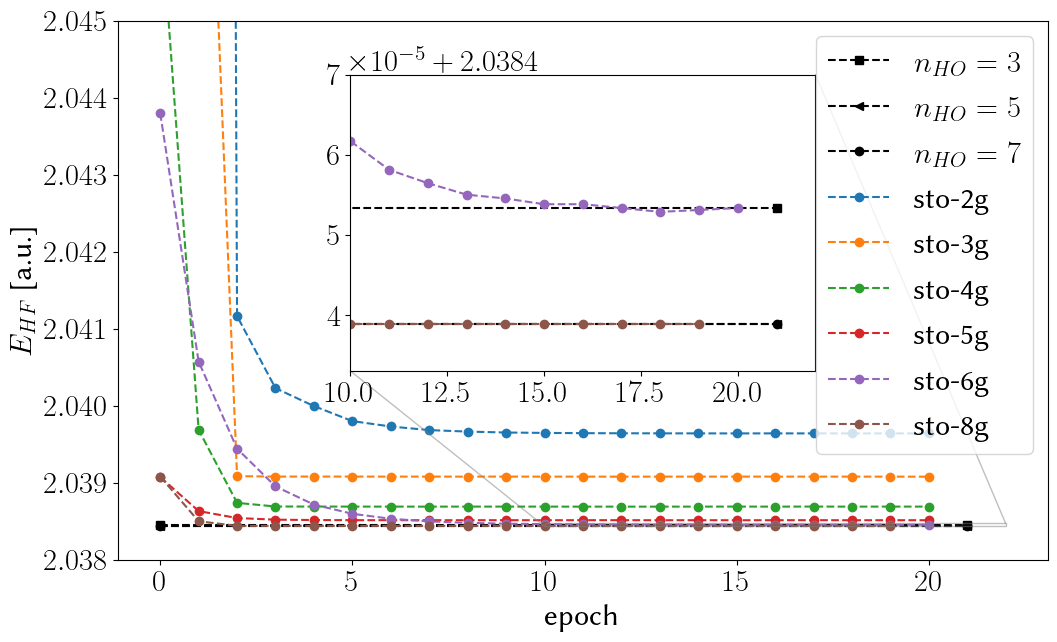
\includegraphics[width=\linewidth]{../plots/HF_optimization}
		\caption{Optimisation of bases with different number of Gaussian basis functions for the Hartree-Fock calculation of Hookium. The exponents $\alpha_{j}$ of the Gaussians were initially set to STO-ng optimised values for the $s$-orbital of Hellium. HF energies calculated using different number of Harmonic Oscillator basis functions $n_{HO}$ are given as reference, values from~\cite{ONeill2003wave}. Learning rate $\alpha=0.1$}
		\label{fig:hfoptimization}
	\end{figure}
	Figure~\ref{fig:hfoptimization} displays the optimisation of bases with different number of Gaussians where the loss is the Hartree-Fock energy. The notation sto-$n$g refers to using the exponents of Slater type orbitals that use $n$ contracted Gaussians and are fit to the $s$-orbital of the helium atom. Figure clearly shows that the optimal exponents for Hookium are different than for helium. In order to achieve the HF limit eight optimized Gaussians were needed, in fact our implementation of variational Hartree-Fock improves on two previous estimates using eight and ten Gaussians~\cite{ONeill2003wave, amovilli2003exact}. A comparison of the results is fund in Table~\ref{tab:HFenergies}.
	\begin{table}[h]
		\centering
		\begin{tabular}{@{}lccl@{}} 
			\toprule
			Basis & Optimised & Source & $E_{HF}$[$Eh$]\\ \midrule
			STO-2g & \cmark & o.w. & 2.039639 \\
			STO-3g & \cmark & o.w. & 2.039077 \\
			STO-4g & \cmark & o.w. & 2.038688 \\
			C-10g & \xmark & \cite{amovilli2003exact} & 2.03851 \\
			STO-5g & \cmark & o.w. & 2.038512 \\
			STO-6g & \cmark & o.w. & 2.038454 \\
			HO-3 & \xmark & \cite{ONeill2003wave} & 2.038453 \\ 
			C-8g & \xmark & \cite{ONeill2003wave} & 2.038439 \\
			C-8g & \cmark & o.w. & 2.038438 \\
			HO-5 & \xmark & \cite{ONeill2003wave} & 2.038438 \\ 
			\bottomrule
		\end{tabular}
		\caption{\label{tab:HFenergies}Hartree-Fock energies with different bases. STO-ng are exponents from optimized Slater orbitals for helium-1s orbital, HO is harmonic oscillator basis and C-ng is $n$ Gaussians with exponents given by $8 / 2^{n-1}$. We see that small numbers of optimised Gaussians outperforms large numbers of unoptimised Gaussians and that HO basis outperforms both.}
	\end{table}
	Thus the correlation energy of the Hookium species with $k=1/4$ is $E_c = -38.4388\cdot 10^{-3} E_h$, which is remarkably similar to other two electron species like He, Li$^+$ ion and Be$^{+2}$ ion. The correlation energy of Hookium supports the claim of Kestner and Sinanoglu that correlation energies of two electron systems are not much effected by the magnitude of the external field~\cite{ONeill2003wave}. A comparison of correlation energies is given in table~\ref{tab:corrs}.
	\begin{table}[h]
		\centering
		\begin{tabular}{@{}cc@{}} 
			\toprule
			Species &  $E_c $ [$E_h$] \\ \midrule
			He			& -0.0420 \\
			Li$^+$		& -0.0435 \\
			Be$^{+2}$	& -0.0443 \\
			Hookium	(k=$\frac{1}{4}$)	& -0.0384 \\
			\bottomrule
		\end{tabular}
		\caption{\label{tab:corrs} Correlation energies for different species~\cite{kais1993density}.}
	\end{table}
	The Hookium model provides a perfect candidate to further explore this claim. We simply solve the the model with the HF method and with VMC at different values of $k$ to see how the correlation energy is influenced by the strength of the external field. By comparison to the ions in table~\ref{tab:corrs} we expect the magnitude of correlation energy to increase slightly with increasing $k$. This is exactly what we see on Figure~\ref{fig:correng}, both the HF $E_{HF}$ and variational $E_V$ energy increase in stronger harmonic confinements and they do so much more rapidly than the difference between the two.
	\begin{figure}[h]
	\centering
	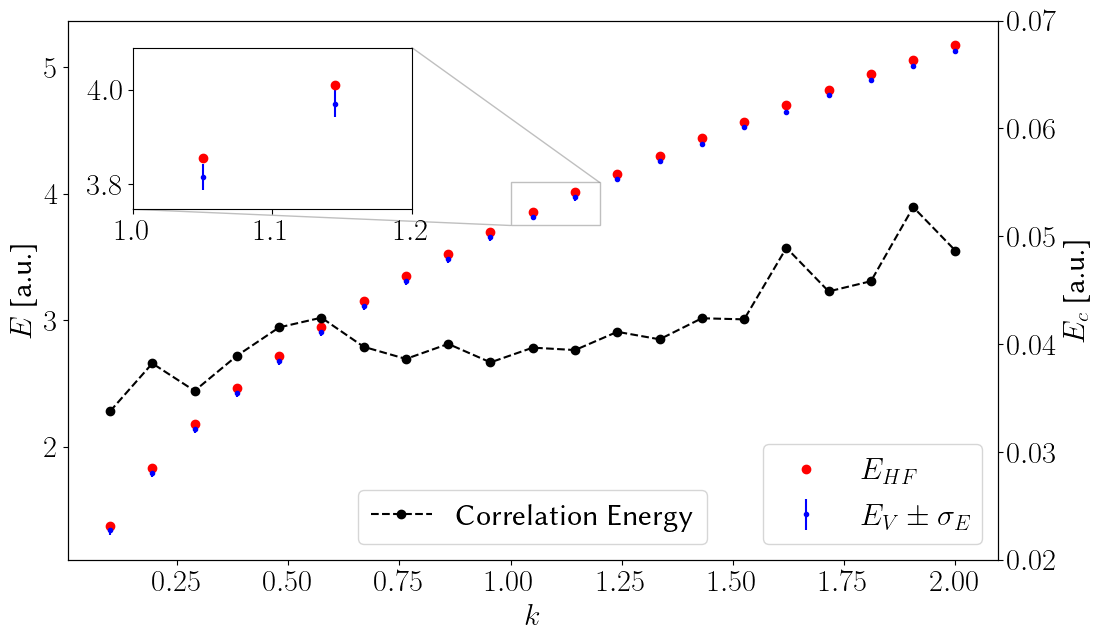
\includegraphics[width=\linewidth]{../plots/corrPlot.png}
	\caption{Correlation energy for different Hooke coefficients $k$. The Hartree-Fock energy was computed with STO-6g basis optimised over $15$ epochs with $\alpha_{HF} = 0.05$ and the true ground state with 1g+J1 basis optimised over $10^3$ epochs with $\alpha=0.005$ and $10^6$ samples.}
	\label{fig:correng}
	\end{figure}



	\subsection{Variational Monte Carlo}
	%	As we will se, the cusp condition at Hookium centers $\frac{d u}{d r} = 0.0$ is automatically fulfilled by both our basis sets.
	Hookium atom has two electrons, the Slater-Jastrow wave function is thus
	\begin{equation}
		\Psi_{T}(\mathbf{r}_1, \mathbf{r}_2) = J(r_{12},\{\beta_{j}\})\left|
		\begin{array}{ll}\psi\left(\mathbf{r}_{1}\right)\left|\uparrow_{1}\right\rangle & \psi\left(\mathbf{r}_{2}\right)\left|\uparrow_{2}\right\rangle \\ \psi\left(\mathbf{r}_{1}\right)\left|\downarrow_{1}\right\rangle & \psi\left(\mathbf{r}_{2}\right)\left|\downarrow_{2}\right\rangle
		\end{array}
	\right|.
	\end{equation}
	We have to differentiate between spin up and down states because electrons with different spins are distinguishable. Since the Hamiltonian does not contain any spin dependent terms, the above Slater determinant simplifies/is equivalent to a simple product state
	\begin{equation}
		\Psi_{T}\left(\mathbf{r}_{1}, \mathbf{r}_{2}\right)=J(r_{12},\{\beta_{j}\})\psi(\mathbf{r}_{1})\psi(\mathbf{r}_{2}).
	\end{equation}
	The single particle states $\psi_i$ need not be complicated to achieve high accuracy for the Hookium system, in fact even a single Gaussian is sufficient, clearly Hookium is an exception rather than a rule and more complicated systems require more complex trial wave functions. Satisfying the cusp conditions on the other hand is crucial, as it massively decreases the variance in local energy, Figure~\ref{fig:blocking+jast} displays two Monte Carlo runs one with a Slater trial wave function and one including the Jastrow factor. The large spikes in local energy in the upper run are due to unresolved electron-electron cusp conditions, i.e. when electrons are very close together the $\propto 1/r_{ij}$ term exhibits the wrong limiting behaviour, limiting the applicability of the trial wave function. Were we studying ordinary matter, where the electrons interact with the nuclei via the Coulomb force, nuclear-electron cusp conditions would need to be met as well. In the case of Hookium there is no cusp when either $r_i = 0$ the gradient is zero however, making Gaussians a very appropriate basis. 
	
	The energy and variance are estimated using a \emph{reblocking} transform, this is done to mitigate the effect of correlation between sampled configurations which systematically underestimates the variance of local energy. Local energies are grouped into blocks and averaged over the block length $N_b$ to obtain the reblocked local energy $E_b$, the reblocked variance is simply the variance of $E_b$'s, the procedure is shown on Figure~\ref{fig:blocking+jast}. 
	Monte Carlo trial moves were generated using a Gaussian perturbation of the current configuration driven by gradient of wavefunction, eq.~\eqref{eq:trialmove}. Timestep $\tau$ of $0.3$ leads to around~$\approx 60\%$ move acceptance rate and was used in all simulations.
	\begin{figure}
	\centering
	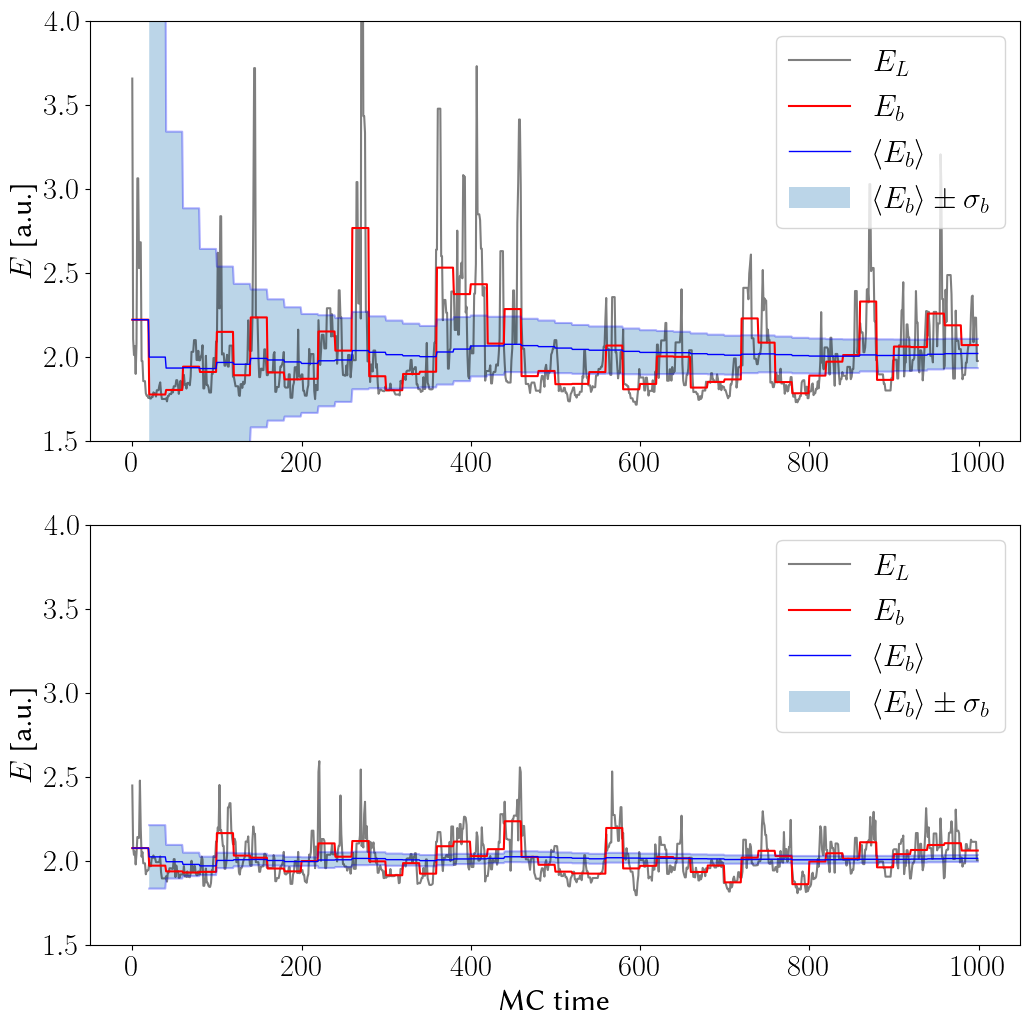
\includegraphics[width=\linewidth]{../plots/blocking.png}
	\caption{Comparison of Monte Carlo local energies $E_L$ from a trial run with (top) Slater trial wave function and (bottom) unoptimised Slater-Jastrow trial wave function. The difference in variance and hence sampling efficiency is evident from the reblocked average energy $\langle E_b \rangle$ and reblocked variance $\sigma_b$.}
	\label{fig:blocking+jast}
	\end{figure}

	Optimisation of the Jastrow factor $J(r_{12}, \{b_j\})$ and the Slater determinant lead to further reduction in variance and energy, but only in the case of variance minimisation. Directly optimising the variational energy proved to be very unstable, this problem was more pronounced when many variational parameters were used, but even for just two optimisable parameters this approach has trouble converging, Figure~\ref{fig:basic-optim}. On the other hand optimizing variance was much more robust, would converge with larger learning rates and needed less samples per epoch for reliable gradients. An optimisation scheme where parameters of the basis (expansion coefficients and exponents) and the Jastrow factor were optimized separately in turns, was tested but it
	\begin{figure*}
		\subfloat[$\rho(\mathbf{r})$, $N=10^3$ samples]{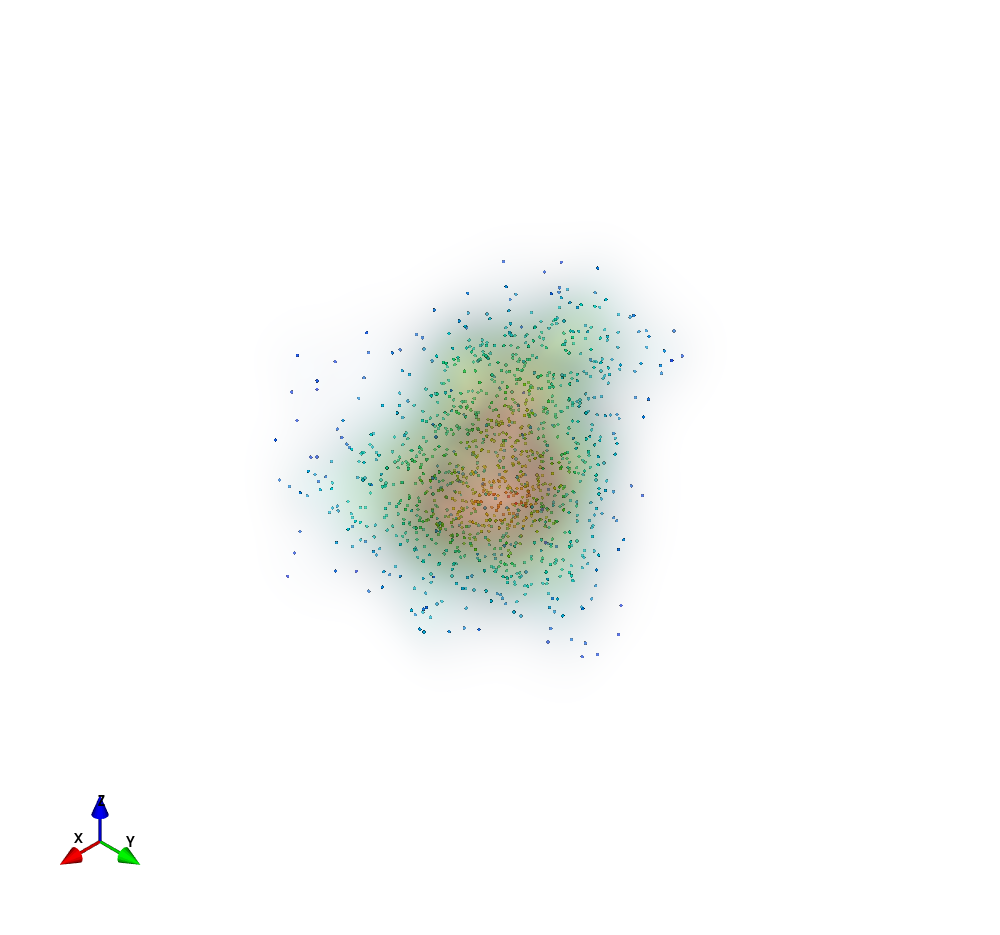
\includegraphics[width = 0.33\linewidth]{../plots/wf-8g-1j-1e3.png}}
		\subfloat[$\rho(\mathbf{r})$, $N=10^4$ samples]{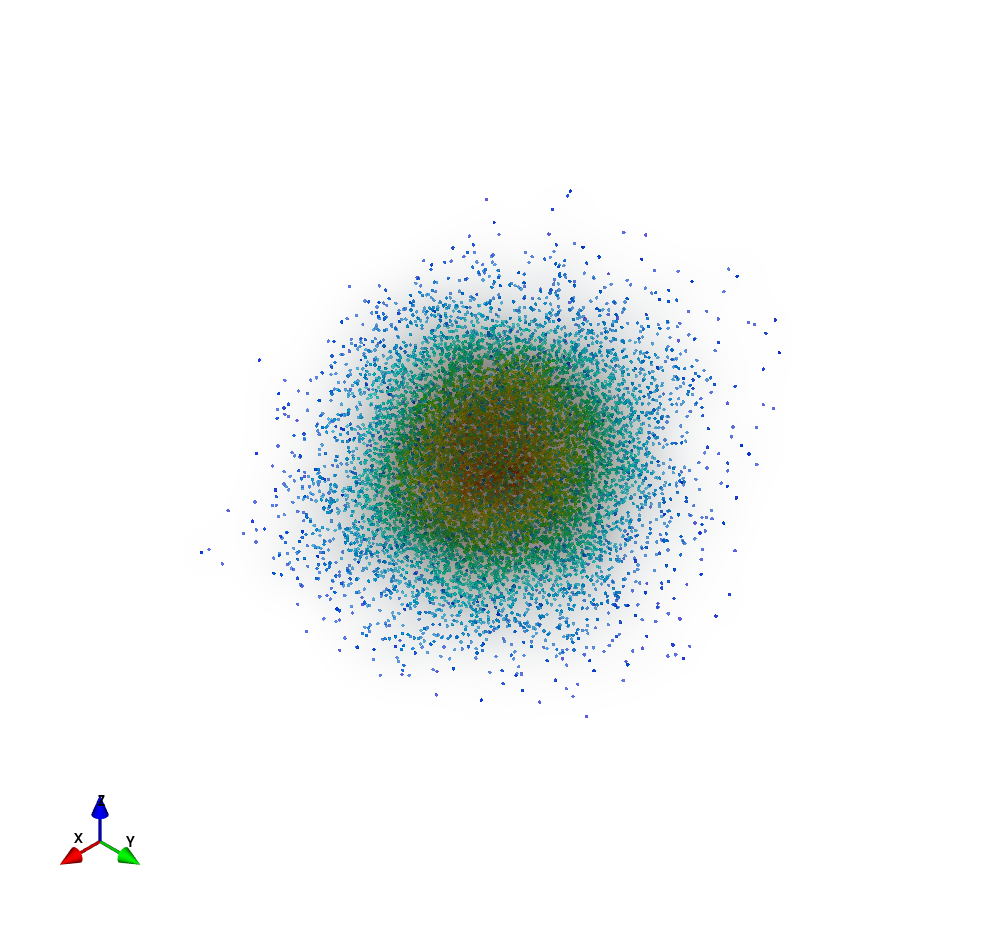
\includegraphics[width = 0.33\linewidth]{../plots/wf-8g-1j-1e4.png}}
		\subfloat[$\rho(\mathbf{r})$, $N=10^5$ samples]{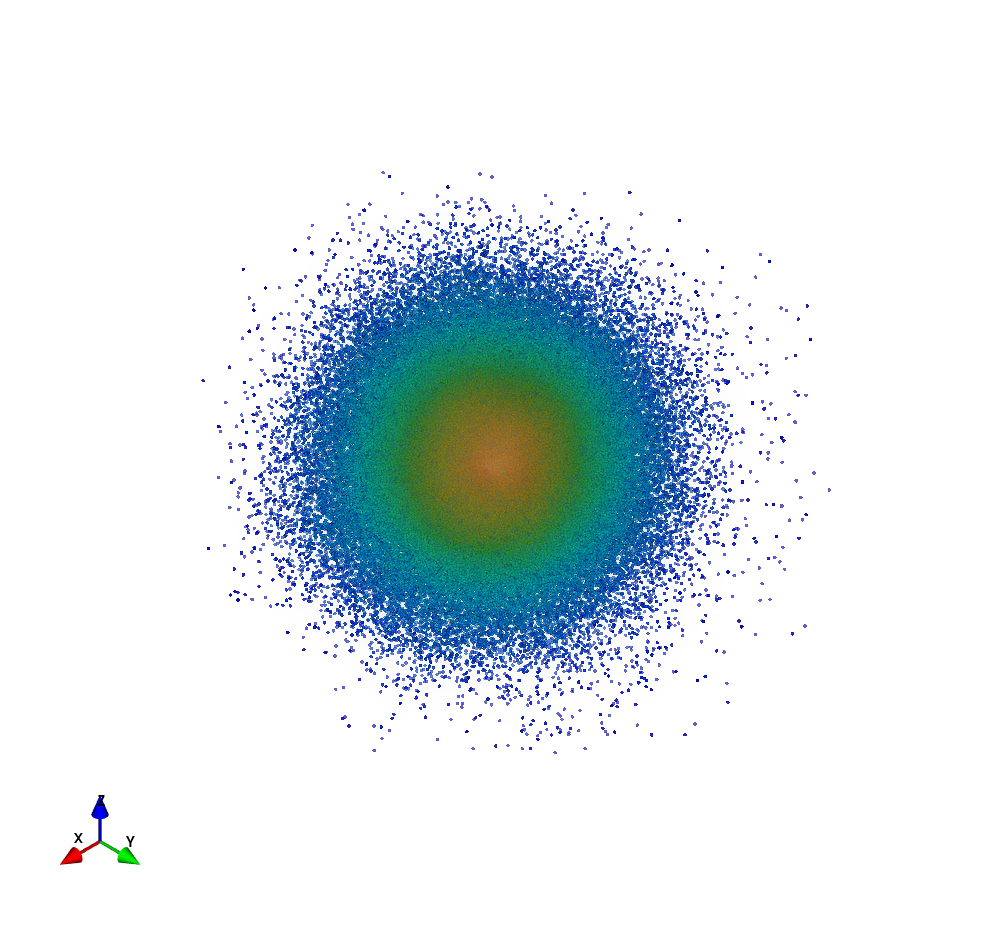
\includegraphics[width = 0.33\linewidth]{../plots/wf-8g-1j-1e5.png}} \\
		\subfloat[$2\pi r^2 \rho(r)$, $N=10^3$ samples]{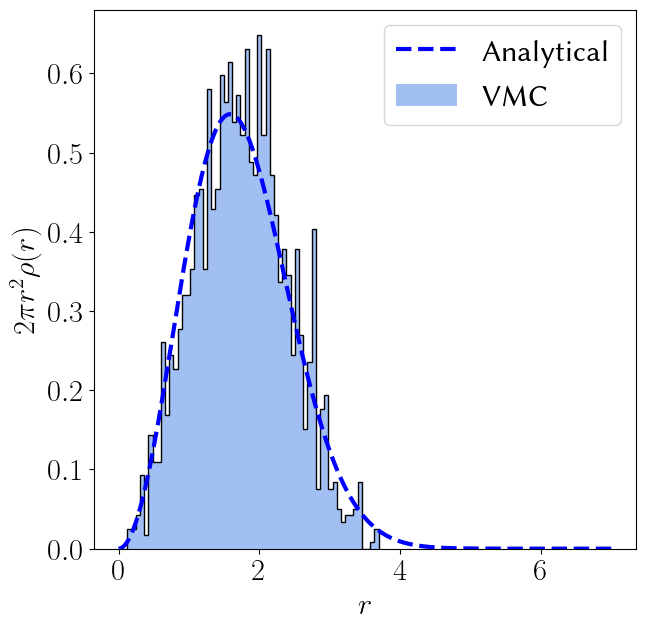
\includegraphics[width = 0.33\linewidth]{../plots/rdens1e3-1g2j.png}} 
		\subfloat[$2\pi r^2 \rho(r)$, $N=10^4$ samples]{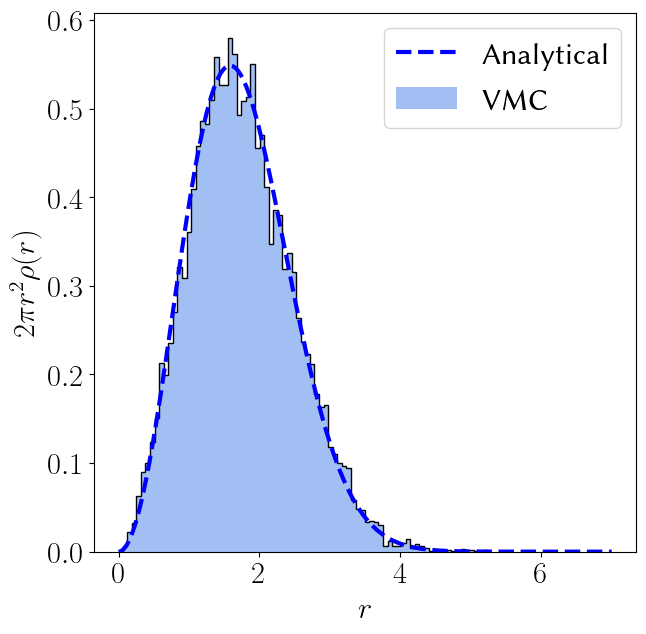
\includegraphics[width = 0.33\linewidth]{../plots/rdens1e4-1g2j.png}}
		\subfloat[$2\pi r^2 \rho(r)$, $N=10^5$ samples]{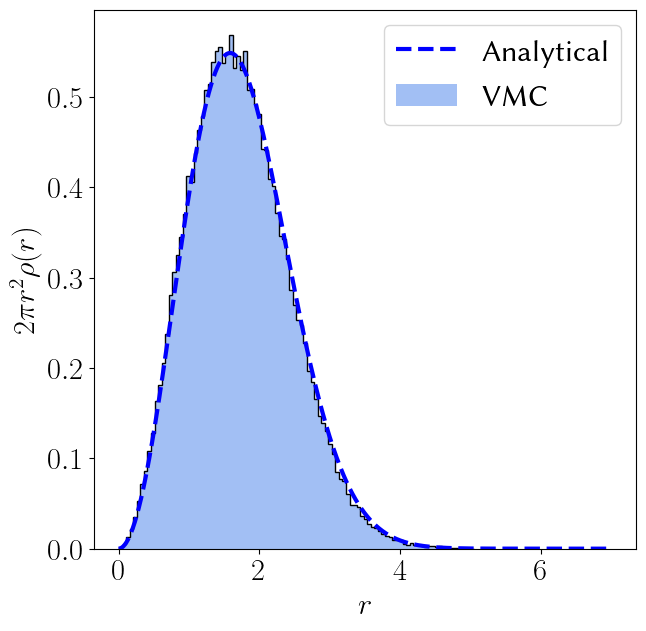
\includegraphics[width = 0.33\linewidth]{../plots/rdens1e5-1g2j.png}} \\
		\subfloat[$P(u)$, $N=10^3$ samples]{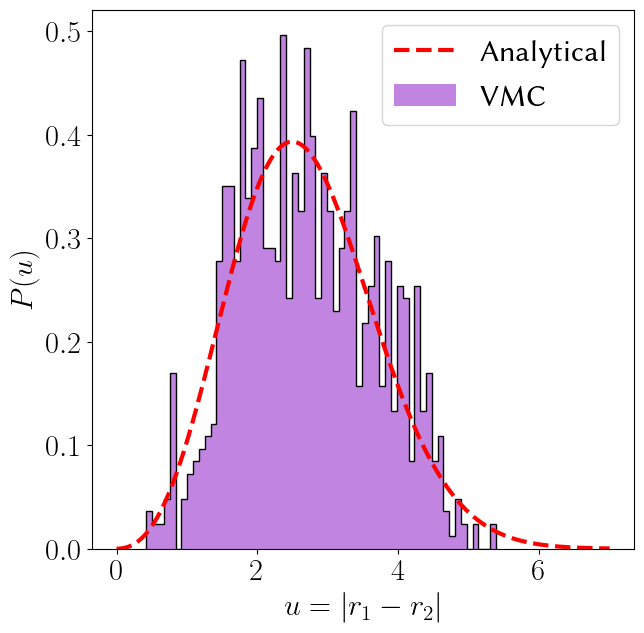
\includegraphics[width = 0.33\linewidth]{../plots/pint1e3.png}} 
		\subfloat[$P(u)$, $N=10^4$ samples]{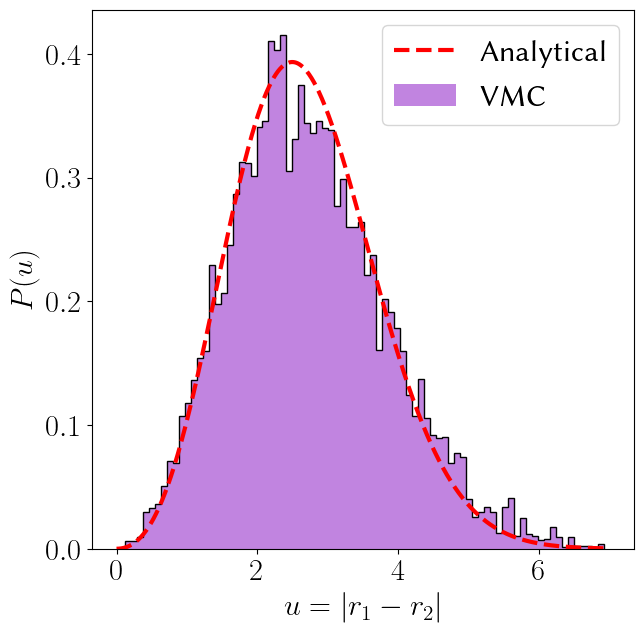
\includegraphics[width = 0.33\linewidth]{../plots/pint1e4.png}}
		\subfloat[$P(u)$, $N=10^5$ samples]{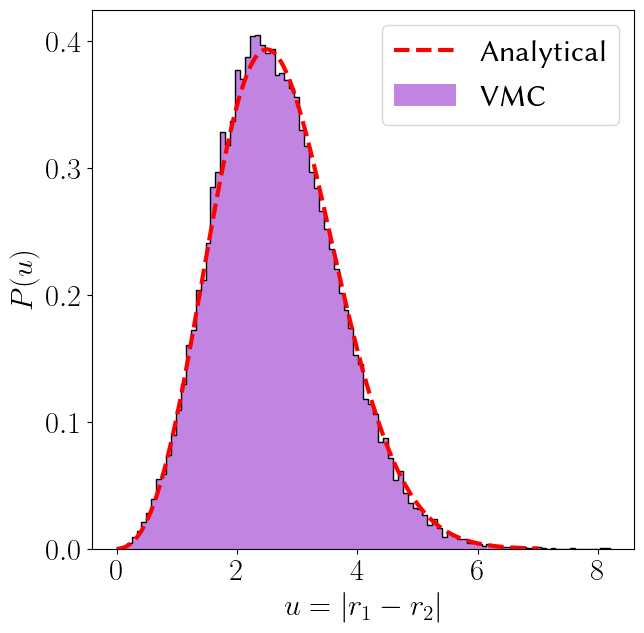
\includegraphics[width = 0.33\linewidth]{../plots/pint1e5.png}}
		\caption{Top row: Electron density of the Hookium atom, sampled from a single Gaussian trial function, with optimised exponent and two term Jastrow factor. Middle row: Radial electron density for a single electron. Bottom row: The position intracule of the samples in top row, compared with the known analytical form.}
		\label{fig:wfsandpints}
	\end{figure*}
	\afterpage{\FloatBarrier}
	\noindent
	did not provide any advantage over optimising all parameters at once.
	
	\begin{figure}
		\centering
		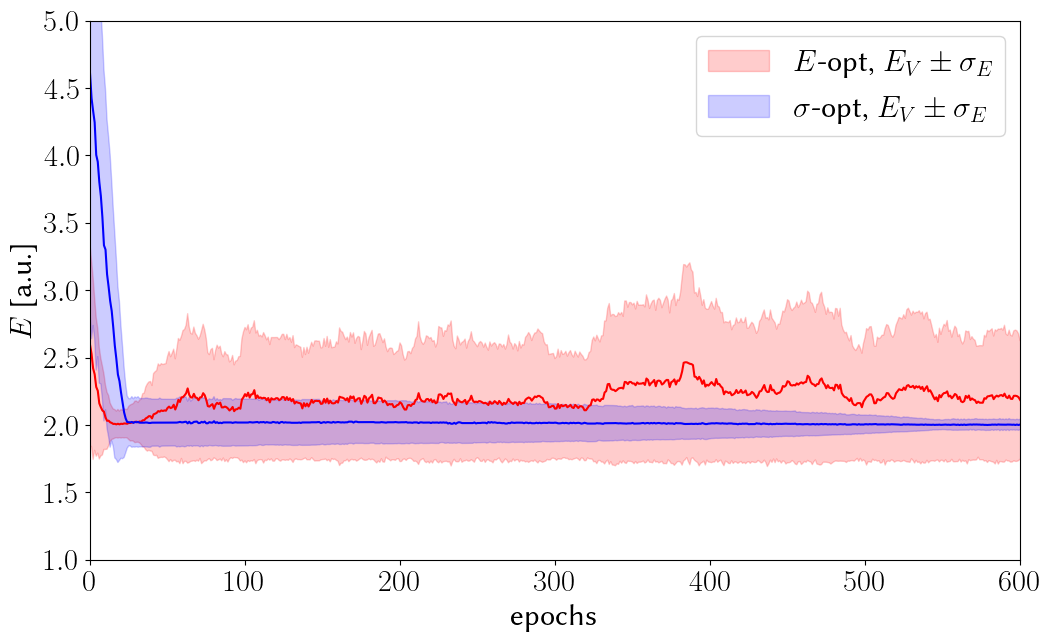
\includegraphics[width=\linewidth]{../plots/vmc-opt-1g.png}
		\caption{Comparison of energy (red) and variance (blue) optimisation of a 1g+J1 trial wave function over 600 epochs with $10^5$ samples. Variance optimisation is much more robust and finds optimal parameters ($\alpha = 0.25, b_{12} = 0.202$) from a very bad initialisation.}
		\label{fig:basic-optim}
	\end{figure}

	When using a Gaussians of only $s$-type orbitals, there is a redundancy in the basis as really only one Gaussian and the Jastrow factor are needed to properly describe Hookium. Moreover, the optimisation procedure reliably found that it is best to set one orbital coefficient to $0.25$ and push all other expansion coefficients $c_{ij}$ towards zero, set all orbital parameters to $0.25$ or a mixture of both. If we use only one Gaussian in the trial wave function and optimise only the Jastrow factor, we see that the factor as given in eq.~\eqref{eq:jast} approaches $(1 + \frac{1}{2}r_{12})$ when we include more terms in expansion~\eqref{eq:u}, depicted on Figure~\ref{fig:jast-optim}.
	
	Simulation results of a VMC simulation with 1g+J2 optimised basis are shown and compared to analytical expressions for the radial electron density and position intracule on Figure~\ref{fig:wfsandpints}. Ground state energies obtained with different bases are presented in Table~\ref{tab:VMCenergies}, our implementation outperforms DFT results using BLYP and BP functionals. Quite importantly blind usage of Hartree-Fock basis (rows 1-4) proved detrimental when studying Hookium, as the exponent parameters of Gaussians that were optimal in HF need not contain an exponent close to $0.25$. If the basis is not optimised during VMC it results in higher energies and variance.
	
	% Address the results in the table

	\begin{figure}
		\centering
		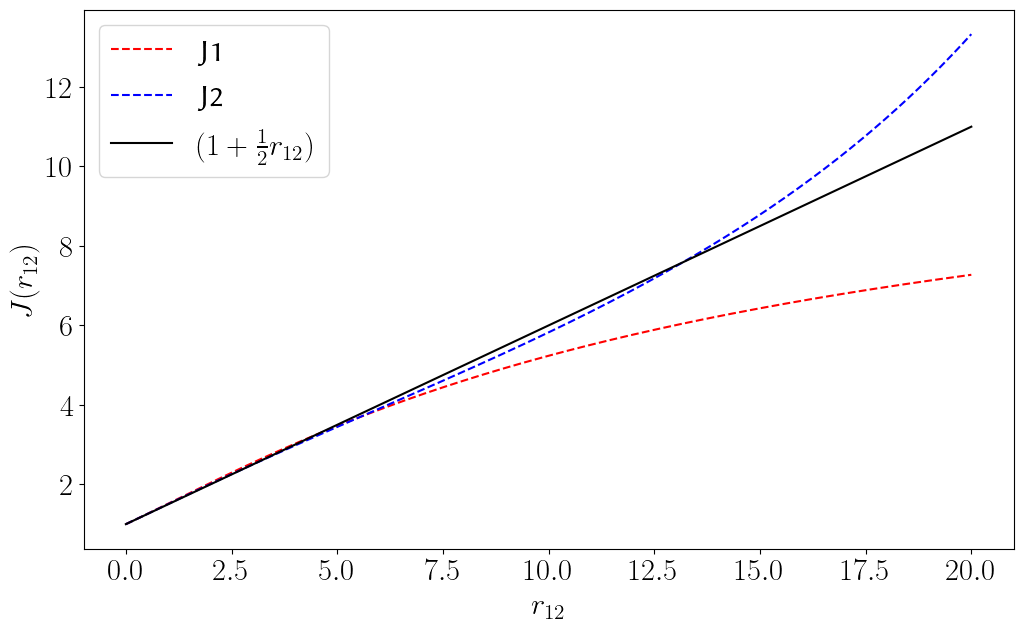
\includegraphics[width=\linewidth]{../plots/jastopt.png}
		\caption{Optimised Jastrow factors for a single Gaussian trial wave function. $J_1$: one $b_{1} = 0.20198$ expansion term and $J_2:$ two $b_1 = 0.22442$, $b_2=-0.00407$ terms.}
		\label{fig:jast-optim}
	\end{figure}
	\begin{table*}
		\centering
		\begin{tabular}{@{}lcccccl@{}} 
			\toprule
			Basis & Optimised & Method & Source & $b^{(1)}_{ij}$ & $b^{(2)}_{ij}$ & $E_V \pm \sigma_E$ [$E_h$]\\ \midrule
			STO-2g + J1 & \xmark & VMC & o.w. & \textbackslash & \textbackslash & 2.375010 $\pm$ 0.783208 \\ 
			STO-2g + J1 & \cmark & VMC & o.w. & -0.06367405 & \textbackslash & 2.144614 $\pm$ 0.508516\\ 
			STO-4g + J1 & \xmark & VMC & o.w. & \textbackslash & \textbackslash & 2.024604 $\pm$ 0.237808 \\ 
			STO-4g + J1 & \cmark & VMC & o.w. & 0.32431903 & \textbackslash & 2.009259 $\pm$ 0.169574\\ 
			1g + J1 	& \cmark & VMC & o.w. & 0.20198098 & \textbackslash & 2.000155 $\pm$ 0.012942\\ 
			1g + J2 	& \cmark & VMC & o.w. & 0.22442447 & -0.00406822 & 2.000112 $\pm$ 0.006640\\
			BLYP 		& \xmark & DFT & \cite{kais1993density} & \textbackslash & \textbackslash & 2.0172 $\pm$ \textbackslash \\ 
			BP			& \xmark & DFT & \cite{kais1993density} & \textbackslash & \textbackslash & 1.9985 $\pm$ \textbackslash \\ 
			\bottomrule
		\end{tabular}
		\caption{\label{tab:VMCenergies}Ground state energies for different trial wave functions, calculated with $10^6$ samples. The second column indicates if the Jastrow factor was optimised, otherwise it was fixed with $a=-\frac{1}{2}$ and $b=1.0$.}
	\end{table*}
	
	\subsection{CPU vs. GPU speedup}
	
	\section{Conclusion}
	\label{sec:conclusion}
	In this paper we have introduced the variational quantum Monte Carlo algorithm and provided an implementation of it, including a Hartree-Fock module for trial wave construction. The method was used to study properties of the Hookium atom and was in good agreement with analytically known results. A single Gaussian basis with the Jastrow factor was found sufficient to describe the ground state of the model and was easiest to optimise. Stochastic optimisation, by computing the gradient of energy variance from the sampled configurations, was stable when used for a handful ($\leq 15$) of variational parameters, minimisation of variational energy was not. 

	\subsection{Future work}
	In this work we were limited to studying one single system but the code was written in such a way that expansions should be straightforward, as it stands the Gaussian basis already implements integrals for non collocated $s$-type Gaussians. The computational bottleneck of the Hartree-Fock module has not been addressed, the generalized eigensolver implementation cannot run on the GPU which limits the applicability of the HF module to larger systems. Speeding up the module as well as including more bases to chose from (i.e. plane waves) would enable us to study more interesting, larger systems. 
	The VMC module could be expanded to automatically generate trial wave functions from the HF basis, for arbitrary numbers of electrons, Jastrow factor functionality would need to be expanded in order to accommodate this. When using the method to study multi atomic systems, geometry optimisation could be implemented without much difficulty, because of JAX's strength in computing gradients. Finally, more advanced optimisation techniques should be explored and the VMC code could be expanded into DMC.
	
	\bibliographystyle{elsarticle-num}
	\bibliography{WA2-references.bib}
	
	\appendix
	\section{Hartree-Fock}
	\label{app:HF}
	Restricted Hartree-Fock is applicable to \emph{closed-shell} systems where there is an even number of electrons that form spin-up and spin-down pairs. The unrestricted Hartree-Fock calculation, where spin is explicitly considered, is only slightly more complicated. Both make use of a Slater determinant state and are solved using self-consistent field iteration. By far the most common approach is to expand single electron states in terms of a basis set, see~\ref{app:basissets}, 
	\begin{equation}
		\psi_{i}(\mathbf{r})=\sum_{j=1}^{n} c_{i j} \phi_{i}(\mathbf{r}).
	\end{equation}
	An \emph{exact} HF calculation gives an upper bound on the ground state energy of the system, this is because it does not contain electron correlation. In practice exact HF energy is not achieved because the basis set is finite. In the restricted case, truncated expansion in terms of a basis set leads to \emph{Roothan-Hall equations}
	\begin{equation}
		\mathbf{F}\mathbf{C} = \mathbf{S}\mathbf{C}\mathbf{\epsilon}.
	\end{equation}
	It is a nonlinear generalized eigenvalue problem, where the \emph{Fock} matrix $\mathbf{F}$ depends on the coefficient matrix $\mathbf{C}$. $\mathbf{S}$ is the \emph{overlap} matrix, essentially containing information of how close the basis set is to orthogonality
	\begin{equation}
		S_{p q}=\int \phi_{p}(\mathbf{r}) \phi_{q}(\mathbf{r}) d \mathbf{r},
	\end{equation}
	and $\mathbf{\epsilon}$ is a diagonal matrix of orbital energies. The density matrix $\mathbf{D}$ can be defined in terms of $\mathbf{C}$ as
	\begin{equation}
		D_{p q}=2 \sum_{a=1}^{\frac{N}{2}} c_{a p} c_{a q},
	\end{equation}
	from which the electron density is easily expressed
	\begin{equation}
		\rho(\mathbf{r})=\sum_{p q} D_{p q} \phi_{p}(\mathbf{r}) \phi_{q}(\mathbf{r}).
	\end{equation}
	The Fock matrix is in the literature usually decomposed into
	\begin{equation}
		\mathbf{F}=\mathbf{H}_{\text {core }}+\mathbf{G},
	\end{equation}
	where $\mathbf{H}_{\text {core }}$ is the sum of the kinetic and potential contributions
	\begin{equation}
		\mathbf{H}_{\text {core }}=\mathbf{T}+\mathbf{V}, 
	\end{equation}
	defined in terms of basis functions as
	\begin{equation}
		T_{p q}=-\frac{1}{2} \int \phi_{p}(\mathbf{r}) \nabla^{2} \phi_{q}(\mathbf{r}) d \mathbf{r}
	\end{equation}
	and
	\begin{equation}
		V_{p q}=\int \phi_{p}(\mathbf{r})
		\left[\sum_{A=1}^{M} 
		V(\mathbf r, \{k_A\})
		\right] \phi_{q}(\mathbf{r}) d \mathbf{r}. 
	\end{equation}
	$\mathbf{G}$ is the two-electron contribution to the Fock operator, defined as
	\begin{equation}
		G_{p q}=\sum_{r s} D_{r s}\left[(p q \mid r s)-\frac{1}{2}(p r \mid s q)\right]
	\end{equation}
	where $(p q \mid r s)$ is the \emph{two-electron} integral, in literature written in \emph{chemists'} notation with round brackets
	\begin{equation}
		(p q \mid r s)=
		\int \frac{
			\phi_{p}\left(\mathbf{r}_{\mathbf{1}}\right) \phi_{q}\left(\mathbf{r}_{\mathbf{1}}\right) \phi_{r}\left(\mathbf{r}_{\mathbf{2}}\right) \phi_{s}\left(\mathbf{r}_{\mathbf{2}}\right)}{\left|\mathbf{r}_{\mathbf{1}}-\mathbf{r}_{\mathbf{2}}\right|} d \mathbf{r}_{\mathbf{1}} d \mathbf{r}_{\mathbf{2}}.
	\end{equation}
	In terms of quantities defined the energy of HF is
	\begin{equation}
		E=\operatorname{Tr}\left(\mathbf{D H}_{\text {core }}\right)+\frac{1}{2} \operatorname{Tr}(\mathbf{D G}).
	\end{equation}
	Roothan-Hall equations are solved by iterating between two steps. In the first step, the Fock matrix is constructed from the density matrix (i.e. expansion coefficients), and in the second a new set of coefficients and consequently a new density matrix is obtained by solving the generalized eigenvalue problem. Repeating the two steps converges the system towards self-consistency.

	\section{Basis sets}
	\label{app:basissets}
	\subsection{Gaussian basis set}
	Cartesian Gaussian-type orbitals (GTOs) are one of the most popular basis sets in computational chemistry. They were introduced as an approximation to Slater-type orbitals (STOs), as they massively simplify evaluations of integrals in from the previous section. Each Slater orbital is approximated by an expansion in Gaussian primitives centered at $\mathbf{r}_A = (x_A, y_A, z_A)$, 
	\begin{equation}
		G_{i j k}(\mathbf{r}, \alpha, \mathbf{A})=(x-x_{A})^{i} (y-y_{A})^{j} (z-z_{A})^{k} e^{-\alpha r_{A}^{2}},
	\end{equation}
	where $i,j,k$ combine into the total angular-momentum quantum number as $l = i+j+k \geq 0$ and $\alpha$ is a variational parameter, usually determined with some least-square fit to relevant Slater orbitals. Gaussians of a given total angular-momentum $l$ form a shell, the \emph{s}-shell is $G_{000}$, \emph{p}-shell are $G_{100}$, $G_{010}$ and $G_{001}$, and so on for \emph{d}, \emph{f}, etc. shells. 
	
	A large body of scientific work exists with regards to efficient evaluation of Gaussian-type orbital integrals arising from Hartree-Fock. Most approaches~\cite{mcmurchie1978one, obara1986efficient} boil down to recursive relations that simplify the kinetic energy $T_{pq}$ and two-electron $(p q \mid r s)$ integrals into overlap integrals $S_{pq}$. The most problematic is the nuclear-electron contribution which is not separable in Cartesian directions and requires special treatment. Even though the implementation of the general GTOs basis set is straightforward it proved to be too much work within the time constraints of this written assignment, it is thus a clear direction for expansion of the code in this work. 

	The integrals simplify considerably if we only consider a single site at $\mathbf{r}_0 = (0, 0, 0)$, which is enough to treat Hookium. The overlap integral $S^{\alpha \beta}_{ijk lmn}\coloneq S[G_{ijk}(\mathbf{r}, \alpha, \mathbf{0}), G_{lmn}(\mathbf{r}, \beta, \mathbf{0})]$ decomposes into separate components along Cartesian axes $S^{\alpha \beta}_{ijk lmn}=S_{il}^{\alpha \beta}S^{\alpha \beta}_{jm}S^{\alpha \beta}_{kn}$ each with closed form solution
	\begin{equation}
		\begin{aligned}
			S_{il}^{\alpha \beta} &= \int_{-\infty}^\infty x^{i+l} e^{-\alpha x^{2}-\beta x^{2}} \mathrm{d}x = \\ & = \frac{1}{2}\left(1 + (-1)^{i+l} \right)\sqrt{\frac{1}{(\alpha + \beta)^{1+i+j}}} \Gamma \left(\frac{1+i+l}{2}\right),
		\end{aligned}
	\end{equation}
	where $\Gamma$ is the gamma function. The integral vanishes for odd sums $i+l$. As in the general case, other integrals will be expressed in terms of overlap integrals for easier evaluation, starting with the nuclear attraction contribution $V^{\alpha \beta}_{ijk lmn}=V_{il}^{\alpha \beta}V^{\alpha \beta}_{jm}V^{\alpha \beta}_{kn}$, for each Cartesian axis we get
	\begin{equation}
		V_{il}^{\alpha \beta} = k \int_{-\infty}^{\infty} x^{i}e^{-\alpha x^{2}} x^2 x^{l}e^{-\beta x^{2}}\mathrm{d}x = k S_{i+2l}^{\alpha \beta} = k S_{il+2}^{\alpha \beta}. 
	\end{equation}
	The kinetic energy matrix elements are simplified with use of the derivative identity
	\begin{equation}
		\frac{\partial}{\partial x} G_{ijk} = iG_{i-1jk} - 2\alpha G_{i+1jk},
	\end{equation}
	consequently 
	\begin{equation}
		\frac{\partial^{2}}{\partial x^{2}} G_{ijk}=4\alpha^{2}G_{i+2jk}-2\alpha(2i+1)G_{ijk}+i(i-1)G_{i-2jk}.
	\end{equation}
	Again, Laplacian operator allows for decomposition into $(xyz)$ components, $T^{\alpha \beta}_{ijk lmn}=T_{il}^{\alpha \beta}T^{\alpha \beta}_{jm}T^{\alpha \beta}_{kn}$ each contributing
	\begin{equation}
		T_{il}^{\alpha \beta} = -\frac{1}{2}\int_{-\infty}^{\infty} x^{i}e^{-\alpha x^{2}} \frac{\partial^{2}}{\partial x^{2}}  \left(x^{l}e^{-\beta x^{2}}\right)\mathrm{d}x,
	\end{equation}
	expressed with overlap integrals
	\begin{equation}
		T_{il}^{\alpha \beta} = -2\beta^{2}S_{il+2}^{\alpha \beta}+\beta(2l+1)S_{il}^{\alpha \beta}-\frac{i}{2}(i-1)S_{il-2}^{\alpha \beta}.
	\end{equation}
	The two-electron integral is the most difficult, it cannot be expressed as a product of integrals for each axis. Closed form solutions for arbitrary angular momenta exist but include a $15$-fold summation and are impractical for anything but $(ss|ss)$ integrals. In practice the expression is evaluated by using a recursive relation to break down high angular momentum integrals into only $(ss|ss)$-type contributions~\cite{fermann2020fundamentals}. We use the Obara-Saika scheme, following notation from notation from~\cite{helgaker1995gaussian}. First we recursively define Hermite Gaussians $E_{t}^{i j}$ as
	\begin{equation}
		\begin{aligned}
			E_{t}^{i j} &= \frac{1}{2 p} E_{t-1}^{i, j-1}+\frac{q Q_{x}}{\beta} E_{t}^{i, j-1}+(t+1) E_{t+1}^{i, j-1} \\ E_{t}^{i j} &=\frac{1}{2 p} E_{t-1}^{i-1, j}-\frac{q Q_{x}}{\alpha} E_{t}^{i-1, j}+(t+1) E_{t+1}^{i-1, j} \\ E_{0}^{00}&=K_{A B} \\ 
			E_{t}^{i j}&=0 \quad \text { if } \quad t<0, \quad \text { or } \quad t>i+j,
		\label{eq:recHermitGauss}
		\end{aligned}
	\end{equation}
	where the auxiliary variables $K_{AB}, Q_x, q, p$ and $P_x$ are defined for two Gaussians with $\alpha$ and $\beta$ at positions $\mathbf{r}_A, \mathbf{r}_B$ as
	\begin{equation}
		\begin{aligned} 
			K_{A B} &=\exp \left(-q Q_{x}^{2}\right) \\ Q_{x} 
			&=x_{A}-x_{B} \\ q 
			&=\frac{\alpha \beta}{\alpha+\beta} \\ p 
			&=\alpha+\beta\\ 
			P_{x} &=\frac{1}{p}\left(\alpha A_{x}+\beta B_{x}\right).
		\end{aligned}
	\end{equation}
	For our simplified case of coinciding only first terms in the recurrence relation~\eqref{eq:recHermitGauss} are nonzero and $K_{AB}=1$. Additionally we need to define the auxiliary Hermite Coulomb integral $R_{t u v}^{n}(p, \mathbf{r}_P, \mathbf{R}_C)$ between Gaussian at $\mathbf{r}_P$ and Coulomb charge center at $\mathbf{R}_C$ as
	\begin{equation}
		\begin{aligned} 
			R_{t+1, u, v}^{n} &=t R_{t-1, u, v}^{n+1}+(x_P - x_C) R_{t, u, v}^{n+1} \\ 
			R_{t, u+1, v}^{n} &=u R_{t, u-1, v}^{n+1}+(y_P - y_C) R_{t, u, v}^{n+1} \\ 
			R_{t, u, v+1}^{n} &=v R_{t, u, v-1}^{n+1}+(z_P - z_C) R_{t, u, v}^{n+1} \\ 
			R_{0,0,0}^{n} &=(-2 p)^{n} F_{n}\left(p R_{P C}^{2}\right).
		\end{aligned}
	\end{equation}
	Again the relations simplify for our case, $F_n$ is the Boys function, a special case of the incomplete Gamma function
	\begin{equation}
		F_{n}(x)=\int_{0}^{1} \exp \left(-x t^{2}\right) t^{2 n} \mathrm{d} t.
	\end{equation}
	The two-body integral $(pq|rs)$ is evaluated as~\cite{helgaker1995gaussian}
	\begin{equation}
		\begin{aligned} (pq|rs)=& \frac{2 \pi^{5 / 2}}{p p^{\prime} \sqrt{p+p^{\prime}}} \sum_{t u v} E_{t u v}^{a b} \sum_{t^{\prime} u^{\prime} v^{\prime}}(-1)^{t^{\prime}+u^{\prime}+v^{\prime}} \\ & \times E_{t^{\prime} u^{\prime} v^{\prime}}^{c d} R_{t+t^{\prime}, u+u^{\prime}, v+v^{\prime}}\left(\alpha, \mathbf{P}, \mathbf{P}^{\prime}\right),
		\end{aligned}
	\end{equation}
	where $p = \alpha + \beta$ and $p^\prime = \gamma + \delta$ are sums of Gaussian exponents. 


	\subsection{Harmonic Oscillator basis set}
	The harmonic Oscillator basis set is composed of eigenfunctions of the Harmonic oscillator in three dimensions
	\begin{equation}
			\phi_{k}(r)=\frac{H_{2 k-1}(r / \sqrt{2})}{2^{k} \sqrt{(2 k-1) !} r / \sqrt{2}} \frac{\exp \left(-r^{2} / 4\right)}{(2 \pi)^{3 / 4}}.
	\end{equation}
	This basis set is not nearly as commonly used as the GTOs, but is a good enough basis set for Hooke's law atom. The integrals required for Hartree-Fock are straightforward to compute and cheap to evaluate, especially with no angular dependence involved, one only needs to use Hermite recurrence relations
	\begin{equation}
		H_{n+1}(x)=2 x H_{n}(x)-H_{n}^{\prime}(x),
	\end{equation} 
	where the derivatives satisfy
	\begin{equation}
		H_{n}^{\prime}(x)=2 n H_{n-1}(x).
	\end{equation}
	The overlap integral is the most straightforward, using orthogonality between the polynomials
	\begin{equation}
		\int_{-\infty}^{\infty} H_{m}(x) H_{n}(x) e^{-x^{2}} d x=\sqrt{\pi} 2^{n} n ! \delta_{n m},
	\end{equation}
	we obtain
	\begin{equation}
		S_{kl}=\int_{0}^{\infty} \phi_{k}(r) \phi_{l}(r) 4\pi r^2 \mathrm{d} r= \delta_{kl}.
	\end{equation}
	The potential matrix element is not much more difficult to compute
	\begin{equation}
		\begin{aligned}
			V_{kl} &=k \int_{0}^{\infty} \phi_{k}(r) r^2 \phi_{l}(r) 4\pi r^2 \mathrm{d} r = \\
				   &=(4k-1) \delta_{kl} + \delta_{kl+1}\sqrt{4k^2-6k+2} \\
				   &\qquad\qquad\quad+\delta_{kl-1}\sqrt{4k^2+2k},
		\end{aligned}
	\end{equation}
	because one uses the recurrence relations once $V_{kl}$ is tridiagonal instead of diagonal. The kinetic integral is a bit more arduous to evaluate and involves several applications of aforementioned recurrence and derivative expressions
	\begin{equation}
		\begin{aligned}
			T_{kl} &= -\frac{1}{2} \int_{0}^{\infty} \phi_{k}(r) \left(\nabla^2 \phi_{l}(r)\right) 4\pi r^2 \mathrm{d} r = \\
			&=\frac{(3+4k)}{8} \delta_{kl} - \frac{1}{4}\delta_{kl+1}\sqrt{\frac{1}{2}(1-3n+2n^2)} \\
			&\qquad\qquad\qquad-\frac{1}{4}\delta_{kl-1}\sqrt{\frac{1}{2}(n+2n^2)}.
		\end{aligned}
	\end{equation}
	The two-electon integral is the toughest to perform, depending on the type of basis function it is solved by using either a multipole expansion for the $\propto \frac{1}{r_{12}}$ term, representing the term using a Laplace transform, or performing the integral in Fourier space. The latter approach works in the case of harmonic-oscillator basis, because the Fourier transform of a product of two basis functions $\phi_k, \phi_j$ is an even polynomial multiplied by an exponential factor. 
	
	%% Authors are advised to submit their bibtex database files. They are
	%% requested to list a bibtex style file in the manuscript if they do
	%% not want to use elsarticle-num.bst.
	
	%% References without bibTeX database:
	
	% \begin{thebibliography}{00}
	
	%% \bibitem must have the following form:
	%%   \bibitem{key}...
	%%
	
	% \bibitem{}
	
	% \end{thebibliography}
	
	
\end{document}

%%
%% End of file `elsarticle-template-num.tex'.
